\documentclass[applsci,article,submit,moreauthors]{Definitions/mdpi}
\usepackage{tabularx}
\usepackage{array}
\firstpage{1}
\pubvolume{1}
\issuenum{1}
\articlenumber{0}
\pubyear{2026}
\copyrightyear{2026}
\datereceived{}
\daterevised{}
\dateaccepted{}
\datepublished{}
\Title{BiLo-NSGA: Project-Level Local Search for Budget-Constrained Power-Grid Portfolio Optimization}
\Author{Yubin Lin, Jingbo Zhang, Xiaoyu Huang, Dishan Yang, Jiyu Li}
\AuthorNames{Yubin Lin, Jingbo Zhang, Xiaoyu Huang, Dishan Yang, Jiyu Li}
\address{Economic and Technological Research Institute of State Grid Fujian Electric Power Co., Ltd., Fuzhou 350000, Fujian, China}
\corres{Correspondence: 18606932711@163.com (Y. Lin)}
\abstract{Utility review boards must select grid investment portfolios under hard annual budgets, yet independent project scores ignore portfolio interactions and generic evolutionary operators do not express changes in review terms. BiLo-NSGA embeds forward insertion, atomic delete--insert substitution, dependency-aware bonuses, and feasibility recovery within non-dominated sorting while recording accepted moves. On a reproducible benchmark with 120 candidates, eight scenarios, and 30 seeds per stochastic method, BiLo-NSGA attains pooled mean hypervolume 0.17190, 1.12\% above NSGA-II. Across five stochastic baselines, it has 37 positive mean differences in 40 comparisons, 36 Holm-significant wins, and no significant loss; 16 gaps against two deterministic scoring rules are descriptive and favor BiLo-NSGA. A 1600-neighbor Pareto local-search control is significantly lower in all eight scenarios. Component evidence is asymmetric: removing forward insertion is harmful in three scenarios under the primary family, although the ablation has the higher pooled mean, whereas atomic substitution and standalone deletion are unresolved. Public reliability and MTEP16 backtests provide descriptive external consistency. The evidence supports project-level local search with scenario-dependent forward-side effects; atomic substitution contributes reviewable replacement semantics rather than a demonstrated accuracy gain.}
\keyword{power grid investment planning; project portfolio selection; budget constraint; multi-objective evolutionary optimization; NSGA-II; local search; decision traceability}
\providecommand{\tightlist}{\setlength{\itemsep}{0pt}\setlength{\parskip}{0pt}}
\begin{document}
\section{Introduction}\label{introduction}

Power systems face substantial capital requirements from renewable integration, storage deployment, feeder automation, and reinforcement backlogs. NERC reliability reports document the consequences associated with delayed investment in specific asset classes. Utilities must choose among reinforcements, automation retrofits, storage, and renewable-support projects spanning many zones and feeders, while annual budgets fund only a subset. Project review therefore becomes a recurring selection problem with a hard budget, conflicting objectives (cost, reliability benefit, renewable accommodation, and execution risk), and inter-project dependencies.

Current review practice balances traceability against portfolio interaction. AHP/TOPSIS-style scoring exposes each ranking step but evaluates projects independently, omitting budget crowding-out, dependency synergies, and conditional marginal value. Multi-objective evolutionary algorithms (MOEAs) search portfolios directly, but generic bit-level variation and unrecorded search trajectories provide limited decision-level provenance. Grid planning departments and investment review boards require both portfolio-level optimization and a reviewable account of the moves producing a recommendation.

BiLo-NSGA retains a standard NSGA-II kernel and changes the variation stage through project-level local search. The forward pass inserts an affordable project while budget slack remains. The backward-side operation is an atomic substitution: it tentatively removes a weak selected project, inserts the strongest affordable replacement, and accepts or rejects the pair as one move. Dependency bonuses guide insertions toward open project groups, deterministic recovery repairs budget violations, and every accepted insertion, substitution, or repair drop is logged. The trail therefore records project decisions rather than abstract numeric perturbations.

The local-operator evidence is asymmetric. Removing forward insertion is harmful in three scenarios under the primary family, but the ablation has the higher pooled mean because other settings move nominally in its favor. Removing atomic substitution raises the pooled mean by 0.61\%, but the contrast remains unresolved under the declared family; replacing it with legacy standalone deletion raises the pooled mean by 0.22\%, and that contrast also remains unresolved. Substitution is retained for review semantics, not claimed as an accuracy mechanism. A budget-indexed cross-scenario diagnostic ranges from a -0.64\% NSGA-II margin at 0.75x to +3.30\% in the 1.20x large-pool-labeled setting. Because scalar weights also vary, this is a boundary description rather than a causal budget effect.

A second obstacle is the scarcity of public grid investment-review records. We therefore construct a reproducible benchmark of 120 candidate projects in six archetypes. The candidates are derived deterministically from RTS-GMLC production-cost data, SimBench distribution-network data, and cached public NERC report metadata. Eight scenarios vary the budget (0.75x--1.20x nominal), candidate-pool composition, and dependency structure. The candidate-derivation pipeline is shared with the methodologically distinct TRACE-MOEA study {[}33{]}; Section 2.4 and the Data Availability statement disclose this relationship.

The contributions of this paper are:

\begin{enumerate}
\def\labelenumi{\arabic{enumi}.}
\tightlist
\item
  \textbf{A budget-aware local search expressed in project-review operations.} BiLo-NSGA defines forward insertion, atomic delete--insert substitution, dependency-aware scoring, and feasibility recovery within non-dominated sorting. Accepted moves are recorded, and 99.6\% of projects appearing in the final front are covered by at least one logged operation (Section 4; Table 4).
\item
  \textbf{A reproducible public benchmark for budget-constrained grid project review.} 120 candidates derived from RTS-GMLC + SimBench + NERC report metadata, eight scenarios, four budget levels, with the full generation code released (Section 3).
\item
  \textbf{A statistically grounded evaluation against seven baselines and ten ablations.} The archive contains 4320 method--scenario invocations. In the inferential family, BiLo-NSGA is 1.12\% above NSGA-II and records 36 significant wins among 40 stochastic-baseline comparisons, with no significant loss. Sixteen deterministic-rule gaps are descriptive. A direct Pareto local-search control is significantly lower in all eight scenarios (Sections 6.1 and 6.7).
\item
  \textbf{Bounded operator attribution and external-consistency checks.} Forward insertion produces the only resolved local-operator gains; contrasts involving atomic substitution and legacy deletion remain unresolved under the declared comparison family, and neither beats the no-backward ablation. NERC and MTEP16 checks provide descriptive alignment rather than confirmatory review validity (Sections 6.3--6.5).
\end{enumerate}

The remainder of the paper is organized as follows. Section 2 reviews related work. Section 3 formalizes the problem and describes the public benchmark. Section 4 presents BiLo-NSGA. Section 5 details the experimental protocol. Section 6 reports results. Section 7 discusses the findings, Section 8 states limitations, and Section 9 concludes.

\begin{center}\rule{0.5\linewidth}{0.5pt}\end{center}

\section{Related Work}\label{related-work}

Our work sits at the intersection of three research threads: budget-constrained combinatorial optimization and project portfolio selection, investment planning and project review practice in power grids, and local-search-enhanced multi-objective evolutionary algorithms (MOEAs). We review each thread in turn and then position BiLo-NSGA against them and against its companion method TRACE-MOEA.

\subsection{Budget-Constrained Combinatorial Optimization and Project Portfolio Selection}\label{budget-constrained-combinatorial-optimization-and-project-portfolio-selection}

Selecting items under a budget is the multi-objective knapsack setting used by Zitzler and Thiele {[}1{]} to compare Pareto-based schemes. Problem-aware search is important in this landscape. Jaszkiewicz {[}2{]} shows that local search over scalarizing functions can improve on purely recombinative MOEAs, a result reviewed by Lust and Teghem {[}3{]} and later knapsack taxonomies {[}4{]}. Many-objective knapsack problems further challenge standard MOEAs {[}5{]}.

Portfolio studies respond with tailored search. Doerner et al.~{[}6{]} apply Pareto ant colony optimization, while Carazo et al.~{[}7{]} model dependencies, schedules, and resource limits with explicit feasibility handling. Energy applications include coupled risk--benefit portfolios {[}8{]} and hybrid exact--heuristic investment planning {[}9{]}. These methods usually enforce budgets after variation through penalties or repair. They do not define the neighborhood itself as insertion under slack, deletion under violation, and substitution near budget parity.

\subsection{Power Grid Investment Planning and Project Review Decision Methods}\label{power-grid-investment-planning-and-project-review-decision-methods}

Grid investment research divides between expansion optimization and multi-criteria review. Optimization studies coordinate transmission and storage {[}10{]}, value reliability through interruption cost {[}11{]}, assess grid-side storage returns {[}12{]}, and balance battery investment against operating benefit {[}13{]}. These formulations usually size a specific asset class from a small set of alternatives rather than select from more than one hundred heterogeneous projects.

Review practice commonly uses AHP {[}14{]} and TOPSIS {[}15{]}. Recent extensions add objective weighting and explainability {[}16{]}, while site-selection reviews show growing use of multi-objective optimization {[}17{]}. MCDM is traceable but scores projects largely independently, so it misses budget crowding-out and dependencies. Simulation-based assessments of substations and commissioning delays {[}18{]} add network context but do not solve the portfolio search. The open gap is therefore a portfolio-aware method with a reviewable decision path {[}19{]}.

\subsection{Local-Search-Enhanced Multi-Objective Evolutionary Algorithms}\label{local-search-enhanced-multi-objective-evolutionary-algorithms}

Hybridizing evolutionary search with local refinement is a long-standing multi-objective strategy. Ishibuchi and Murata {[}20{]} apply weighted-sum local moves after genetic variation, while Knowles and Corne {[}21{]} show that a \((1+1)\) local search with a Pareto archive can approximate nondominated fronts competitively. NSGA-II {[}22{]}, MOEA/D {[}23{]}, and NSGA-III {[}24{]} rely primarily on selection and recombination; Neri and Cotta {[}25{]} survey the many memetic extensions built around them.

Power-system studies apply improved NSGA-II variants to distribution-network co-optimization {[}26{]}, offshore-wind storage configuration {[}27{]}, and resilient backbone-grid planning {[}28{]}. Enhanced swarm methods address storage planning {[}29{]} and transmission expansion {[}30{]}. These methods modify initialization, operators, or stages, but their local moves, when present, remain numeric perturbations inherited from continuous benchmarks.

Portfolio-scheduling studies also combine NSGA-II with Pareto local search {[}31{]}. More recent methods tailor local refinement to cardinality and pre-assignment constraints {[}32{]}. However, these hybrids neither express moves as adding, removing, or substituting a reviewable project nor retain the accepted move sequence. BiLo-NSGA treats that domain-level trajectory as a traceable output.

\subsection{Relation to TRACE-MOEA and Gap Statement}\label{relation-to-trace-moea-and-gap-statement}

TRACE-MOEA {[}33{]} addresses power-grid project review through preference-adaptive ranking, review-rule repair, and a trace archive. Its contribution acts at selection and ranking. BiLo-NSGA instead changes variation through forward insertion, atomic substitution, dependency-aware bonuses, and feasibility recovery. The two studies share the versioned candidate generator and the public NERC and MTEP16 source corpora. Their problem objectives, algorithm implementations, scenario definitions, run archives, selected portfolios, and reported comparisons are paper-specific.

The resulting gap is specific. Existing knapsack MOEAs generally handle budgets through penalties or post-variation repair. Grid MCDM is traceable but portfolio-blind, and memetic MOEAs express refinement numerically rather than as reviewable project decisions. BiLo-NSGA combines non-dominated sorting with forward insertion, atomic replacement, feasibility recovery, and a per-move decision trace. The claim concerns this intersection rather than universal superiority over memetic optimization.

\begin{center}\rule{0.5\linewidth}{0.5pt}\end{center}

\section{Problem Formulation and Public Benchmark}\label{problem-formulation-and-public-benchmark}

\subsection{Budget-Constrained Portfolio Review as Multi-Objective Selection}\label{budget-constrained-portfolio-review-as-multi-objective-selection}

Let \(\mathcal{C} = \{c_1, \dots, c_n\}\) be the candidate pool. Each project has cost \(k_i\), reliability benefit \(r_i\), renewable-accommodation benefit \(g_i\), load-support value, compliance and evidence scores, and schedule and implementation risks combined as \(\rho_i\). A dependency-group label links projects from the same zone- or feeder-level program. A review decision is a binary vector \(x \in \{0,1\}^n\), where \(x_i = 1\) means project \(c_i\) is funded. The review board's problem is:

\[
\min_{x \in \{0,1\}^n} \; F(x) = \Big( \textstyle\sum_i k_i x_i, \;\; -\sum_i r_i x_i, \;\; -\sum_i g_i x_i, \;\; \frac{\sum_i \rho_i x_i}{\max(1, \sum_i x_i)} \Big)
\]

subject to the \textbf{hard budget constraint}

\[
\textstyle\sum_i k_i x_i \le B,
\]

with normalized constraint violation

\[
v_B(x)=\max\!\left\{0,\frac{\sum_i k_i x_i-B}{B}\right\}.
\]

The four minimization objectives are thus total cost, negated reliability benefit, negated renewable benefit, and mean per-project risk. The budget is not a soft preference: portfolios exceeding \(B\) are not fundable, which is why the benchmark evaluates only the feasible non-dominated front (Section 5.3) and why the method design treats budget slack and violation as first-class quantities that shape the search neighborhood (Section 4).

A portfolio \(x\) dominates \(x'\) when it is at least as good in all four objectives and better in at least one. The non-dominated front contains mutually non-dominating portfolios returned by a method. Hypervolume measures the objective-space volume dominated by that front relative to a fixed reference point, rewarding both convergence and diversity.

\subsection{Benchmark Construction from Public Data}\label{benchmark-construction-from-public-data}

Because real utility investment-review records are institution-internal and unavailable for publication, we derive a candidate pool deterministically from three public sources (Table 1). The full derivation code is released; every rule below is inspectable.

\begin{table*}[t]
\centering
\footnotesize
\setlength{\tabcolsep}{3pt}
\caption{Candidate pool composition.}\label{tab:1}
\begin{tabularx}{\textwidth}{@{}>{\raggedright\arraybackslash}X >{\raggedright\arraybackslash}X >{\raggedright\arraybackslash}X >{\raggedright\arraybackslash}X@{}}
\toprule
Source & Public artifact used & Candidates & Archetypes (kind) \\
\midrule
RTS-GMLC & bus/branch/generator source data, zone-level aggregates & 72 & transmission reinforcement; reliability automation; renewable support \\
SimBench & complete mixed network (\texttt{1-complete\_data-mixed-all-0-sw}), 16 highest-stress subnets & 48 & distribution (feeder) reinforcement; storage flexibility; protection automation \\
NERC / C2GES report cache & metadata of 40 cached public reliability documents (28 event reports) & attribute adjustment only & --- \\
\textbf{Total} &  & \textbf{120} & 6 kinds \\
\bottomrule
\end{tabularx}
\end{table*}

RTS-GMLC zone-level aggregates of load, branch ratings, permanent-outage rates, generator capacity, and renewable share generate three candidate archetypes per zone. Analytic functions map these aggregates to costs and benefits; for example, reinforcement benefit scales with outage pressure, while renewable-support benefit scales with the gap between load and installed renewable capacity. From SimBench, the sixteen subnets with the highest combined load and line-length stress each yield feeder-reinforcement, storage-flexibility, and protection-automation candidates. Their attributes depend on subnet load, line count, and the distributed-energy-resource gap. NERC report metadata then adjusts attributes at the project-kind level. Candidates in the same zone or feeder share a dependency group, producing 120 candidates in six kinds with a block structure.

We emphasize what this construction is and is not. It is a \emph{reproducible, public, engineering-plausible proxy} for the review problem -- every attribute traces to public grid statistics or public reliability-report metadata through published rules. It is not a set of expert-labeled review outcomes, and its cost coefficients are in synthetic cost units, not calibrated currency (Section 8).

\subsection{Review Scenarios}\label{review-scenarios}

Eight experiments exercise the pool along three axes -- budget envelope, pool composition, and dependency structure -- while the evaluation itself (objectives, hypervolume computation) is identical across experiments (Table 2). The nominal budget is \(B = 1020\) cost units.

\begin{table*}[t]
\centering
\footnotesize
\setlength{\tabcolsep}{3pt}
\caption{The eight review scenarios. Pool filters restrict candidate kinds; the evaluation never changes.}\label{tab:2}
\begin{tabularx}{\textwidth}{@{}>{\raggedright\arraybackslash}X >{\raggedright\arraybackslash}X >{\raggedright\arraybackslash}X@{}}
\toprule
Experiment & Budget multiplier & Candidate pool \\
\midrule
budget\_constrained\_selection & 0.88x & full pool (120) \\
reliability\_prioritized\_review & 1.00x & reliability-related kinds only \\
renewable\_accommodation\_review & 1.00x & renewable/storage kinds only \\
dependency\_constrained\_review & 1.00x & candidates in dependency groups of size >= 2 \\
local\_move\_explainability & 1.00x & full pool \\
ranking\_robustness & 1.00x & full pool \\
budget\_sensitivity & 0.75x & full pool \\
project\_pool\_scalability & 1.20x & full pool \\
\bottomrule
\end{tabularx}
\end{table*}

Five experiments use the full candidate pool at budget multipliers 0.75x, 0.88x, 1.00x, 1.00x, and 1.20x. Their labels also alter scalar weights used by some methods, and their random streams are independent. Section 6.2 therefore treats them as a budget-indexed cross-scenario diagnostic rather than a controlled budget-only experiment.

\subsection{Shared Public Benchmark Statement}\label{shared-public-benchmark-statement}

The Section 3.2 candidate pipeline is shared with TRACE-MOEA {[}33{]}. Both studies also use the same public NERC corpus and MTEP16 source records for separately executed consistency checks. Problem objectives, method implementations, scenarios, run records, selected portfolios, and reported comparisons are specific to each paper.

\begin{center}\rule{0.5\linewidth}{0.5pt}\end{center}

\section{BiLo-NSGA}\label{bilo-nsga}

Figure 1 places two project-vocabulary moves between global offspring generation and dependency-aware feasibility recovery. Forward insertion spends useful slack. Atomic substitution removes one weak selection and evaluates one affordable replacement before either change can be committed. The candidates then compete under the same constrained non-dominated sorting rule as the baseline kernel. Forward insertion produces the only significant local-operator gains; substitution supplies review semantics without a demonstrated hypervolume gain.

\begin{figure*}[t]
\centering

\includegraphics[width=0.94\textwidth]{figures/fig_architecture.png}
\caption{BiLo-NSGA architecture. The feedback arrow denotes the next generation. The lower strip identifies sensitivity and external-consistency analyses rather than optimization inputs.}\label{fig:1}
\end{figure*}

BiLo-NSGA is a memetic multi-objective algorithm: a standard non-dominated sorting kernel provides global search and Pareto pressure, and project-vocabulary local moves provide budget-aware intensification and recorded decision events. Each component below is individually switchable, enabling the one-switch and legacy-rule comparisons in Section 6.3.

\textbf{Formal definitions.} Let \(x\in\{0,1\}^{n}\) and define remaining budget and violation as

\[
s_B(x)=B-\sum_{j=1}^{n}c_jx_j,\qquad
v_B(x)=\max(0,-s_B(x)).
\]

With normalized minimized objectives, the acceptance scalar used \emph{inside local search only} is

\[
\Phi(x)=\sum_{q=1}^{Q}\omega_q\tilde f_q(x)+\lambda v_B(x).
\]

For an unselected affordable project, the dependency-aware insertion score is

\[
R_j^{+}(x)=\frac{\sum_q\omega_q b_{jq}}{c_j}
\left[1+0.06\,\mathbb I\!\left(\exists \ell:x_\ell=1,\ d_\ell=d_j\right)\right].
\]

The forward proposal and acceptance rule are

\[
j^+=\operatorname*{arg\,max}_{j:x_j=0,\ c_j\leq s_B(x)}R_j^+(x),
\qquad x^+=x+e_{j^+},
\]

\[
x\leftarrow x^+\quad\text{iff}\quad \Phi(x^+)<\Phi(x);
\quad\text{otherwise the forward pass stops.}
\]

For atomic substitution, first select a removal candidate

\[
j^-=\operatorname*{arg\,min}_{j:x_j=1}
\frac{\sum_q\omega_q b_{jq}}{c_j},\qquad x^-=x-e_{j^-}.
\]

The affordable replacement set excludes that project,

\[
\mathcal A(x^-)=\{j:x^-_j=0,\ j\neq j^-,\ c_j\leq s_B(x^-)\},
\]

and \(j^+=\operatorname*{arg\,max}_{j\in\mathcal A(x^-)}R_j^+(x^-)\). The pair is atomic:

\[
x\leftarrow x-e_{j^-}+e_{j^+}
\quad\text{iff}\quad
\mathcal A(x^-)\neq\varnothing\ \land\ |x^-|\geq2\ \land\
\Phi(x-e_{j^-}+e_{j^+})<\Phi(x).
\]

Otherwise both tentative edits are rolled back and the pass stops. Thus the proposed method never accepts a standalone backward deletion; that legacy rule is retained only as a named ablation.

Feasibility recovery applies the same deletion ranking without the improvement test until \(v_B(x)=0\). For local depths \(D_+\) and \(D_-\), a direct scan implementation costs

\[
T_{\mathrm{local}}=O\!\left((D_++D_-)nQ\right)
\]

per selected offspring, in addition to objective evaluation. The current implementation uses \(D_+=8\), \(D_-=4\); this complexity expression does not imply that both directions produce equal empirical benefit.

\subsection{Non-Dominated Sorting Kernel}\label{non-dominated-sorting-kernel}

The kernel is a binary NSGA-II with uniform crossover and bit-flip mutation at rate \(1/n\). Constraint dominance ranks feasible solutions above infeasible ones and compares infeasible solutions by violation. Crowding distance truncates the population to 40 over 40 generations. Keeping this standard kernel isolates the proposed contribution in the variation stage.

\subsection{Forward Insertion}\label{forward-insertion}

After variation, half of the offspring undergo a forward pass of depth at most eight. While slack remains, the affordable unselected project with the highest equal-weight benefit-to-cost ratio is tentatively inserted. The insertion is retained only if it improves normalized scalarized fitness, defined as the sum of normalized objectives plus a violation penalty. The pass stops at the first rejection. This move converts budget slack left by recombination into a candidate improvement.

\subsection{Atomic Backward--Forward Substitution}\label{atomic-backwardforward-substitution}

The substitution pass has depth at most four. It removes the selected project with the lowest benefit-to-cost ratio only provisionally, uses the released budget to choose the highest-scoring affordable replacement, and evaluates the resulting portfolio once. Acceptance commits both edits; rejection restores both. The pass stops at the first rejection and never proposes from a portfolio with fewer than two retained projects. This construction makes replacement reviewable as one decision rather than inferring it from unrelated insert and delete events. Section 6.3 shows that the semantic improvement does not yield a significant hypervolume change.

\subsection{Dependency-Aware Move Bonus}\label{dependency-aware-move-bonus}

When ranking insertion candidates, the benefit-to-cost score is multiplied by 1.06 if another member of the candidate's dependency group is already selected. The bonus represents the possibility that related investments, such as reinforcement and automation on the same feeder, form a coherent program. Section 6.3 treats the dependency-density control as a direct test of this design choice.

\subsection{Feasibility Recovery}\label{feasibility-recovery}

Every initial or offspring portfolio that violates the budget is repaired deterministically. The selected project with the lowest benefit-to-cost ratio is removed until the portfolio is affordable. Because each step removes one selected project and the empty portfolio is feasible, repair terminates after at most \(\|x\|_0\) drops. Each restoration step is recorded in the decision trace.

\subsection{Per-Move Decision Trace}\label{per-move-decision-trace}

Every accepted move--\texttt{forward\_insert}, \texttt{backward\_substitute}, and \texttt{repair\_drop}--is logged with its generation and project identifier(s). A substitution record stores both the removed and inserted project. The trail is a pure output: no trace statistic enters any objective, constraint, or selection decision. BiLo-NSGA logs on average 3668 moves per run, and 99.6\% of projects appearing in the final non-dominated front are covered by at least one logged move (Table 4). These values measure archive production, not explanation quality.

\subsection{Algorithm Summary}\label{algorithm-summary}

\begin{verbatim}
BiLo-NSGA(pool, budget, seed):
  initialize population of 40 sparse random portfolios; repair each to budget   # 4.5
  for gen = 1 .. 40:
    offspring <- uniform crossover + bit-flip mutation (rate 1/n)               # 4.1
    for each offspring:
      repair to budget (log repair_drop moves)                                  # 4.5
      if selected for local search (half of offspring):
        forward pass  (depth <= 8): insert best affordable BCR candidate,       # 4.2
                      dependency bonus 1.06 on open groups,                     # 4.4
                      keep only fitness-improving inserts (log forward_insert)
        substitution pass (depth <= 4): tentatively remove worst-BCR item,     # 4.3
                      insert best affordable replacement, accept pair only
                      if fitness improves (log backward_substitute)
    environmental selection: constraint-dominated NDS + crowding (top 40)       # 4.1
  return feasible non-dominated front + decision trace                          # 4.6
\end{verbatim}

\begin{center}\rule{0.5\linewidth}{0.5pt}\end{center}

\section{Experimental Setup}\label{experimental-setup}

\subsection{Methods Compared}\label{methods-compared}

Table 3 lists the eighteen methods: BiLo-NSGA, seven baselines spanning evolutionary, Pareto-local-search, and MCDM families, and ten ablations. The evolutionary baselines are reference implementations from pymoo on the identical binary-encoded, budget-constrained problem. Pareto Local Search uses add, delete, and swap neighborhoods with a fixed budget of 1600 evaluated neighbors per run.

\begin{table*}[t]
\centering
\scriptsize
\setlength{\tabcolsep}{3pt}
\caption{Methods.}\label{tab:3}
\begin{tabularx}{\textwidth}{@{}>{\raggedright\arraybackslash}X >{\raggedright\arraybackslash}X >{\raggedright\arraybackslash}X@{}}
\toprule
Method & Role & Description \\
\midrule
BiLo-NSGA & proposed & NSGA-II core + forward insertion + atomic substitution + dependency moves + feasibility recovery \\
NSGA-II & baseline & pymoo NSGA-II, binary encoding, constrained \\
NSGA-III & baseline & pymoo NSGA-III with Das-Dennis reference directions \\
MOEA/D & baseline & pymoo MOEA/D, budget as penalty \\
Greedy BCR & baseline & benefit-cost-ratio greedy fill under budget \\
AHP-TOPSIS & baseline & AHP-derived weights + TOPSIS ranking + greedy fill \\
Random Feasible & baseline & random permutation greedy fill \\
Pareto Local Search & baseline & multi-start add/delete/swap Pareto local search; 1600-neighbor budget \\
Ablation-NoForwardSearch & ablation & forward insertion disabled \\
Ablation-NoBackwardSearch & ablation & atomic substitution disabled \\
Ablation-LegacyDeletion & ablation & atomic substitution replaced by standalone greedy deletion \\
Ablation-RandomMutationOnly & ablation & local search replaced by high-rate (3/n) random mutation \\
Ablation-NoDependencyMoves & ablation & dependency-aware move bonus disabled \\
Ablation-NoFeasibilityRecovery & ablation & budget repair disabled \\
Ablation-WeightedRankingOnly & ablation & weighted ranking without evolution \\
Ablation-ShallowLocalSearch & ablation & local-search depth reduced to 2 \\
Ablation-LowDependencyDensity & ablation & dependency graph thinned (every 3rd candidate isolated) \\
Ablation-LooseBudget & ablation & search at 1.2x budget, evaluated at the true budget \\
\bottomrule
\end{tabularx}
\end{table*}

Each ablation flips exactly one switch relative to the full method; the last two are stress variants that perturb the dependency structure and the search budget rather than removing an operator, and we read them as robustness probes.

\subsection{Protocol}\label{protocol}

The rectangular archive contains \textbf{18 methods x 8 experiments x 30 invocations = 4320 rows}. Fourteen opponents are stochastic. AHP-TOPSIS, Greedy BCR, and Ablation-WeightedRankingOnly are deterministic; their repeated identical invocations are retained for provenance but have effective sample size one per experiment. All evolutionary methods use population 40 and 40 generations. Pareto Local Search receives a numerical ceiling of 1600 evaluated neighbors, matching the nominal \(40\times40\) offspring-evaluation ceiling but not computational work; wall-clock runtime is reported separately. Preference weights used by scalarizing methods never enter the evaluation metric.

\subsection{Evaluation Metric and Statistics}\label{evaluation-metric-and-statistics}

Portfolio quality is measured by the \textbf{standard hypervolume} of the feasible non-dominated front. Objective values are normalized with \emph{fixed per-problem bounds} computed once per experiment from a seeded reference set (the empty portfolio, all single-project portfolios, and 2048 random feasible portfolios), and the reference point is \(1.1\) in every normalized dimension. An empty feasible front scores zero. The metric contains no method-aware ingredient, and decision-trace statistics such as move counts and coverage are reported descriptively rather than entering any ranking.

Statistical comparisons use two-sided \textbf{Mann--Whitney U tests} between BiLo-NSGA and each of the fourteen stochastic opponents per experiment (\(n=30\) per group), with \textbf{Holm correction} within each stochastic family. We report rank-biserial effects and 5000-resample bootstrap confidence intervals for mean differences. The three deterministic rules are compared descriptively and receive no seed-level p-values. The corrected table is \texttt{real\_project\_review\_inference\_v2.csv}; the original rectangular significance output remains only as provenance.

The method-independent normalization for objective \(j\) is

\[
\tilde f_j(x)=\min\!\left\{1,\max\!\left[0,\frac{f_j(x)-l_j}{u_j-l_j}\right]\right\},
\]

where \((l_j,u_j)\) comes from the frozen reference sample rather than any compared method. The scored set for method \(m\), experiment \(e\), and seed \(r\) is

\[
\mathcal{P}_{mer}=\left\{x\in\mathcal{X}_{mer}:v_B(x)=0,\ \nexists y\in\mathcal{X}_{mer}\text{ with }\tilde F(y)\prec\tilde F(x)\right\}.
\]

Its standard four-objective hypervolume is

\[
HV(\mathcal{P}_{mer})=\lambda_4\!\left(\bigcup_{x\in\mathcal{P}_{mer}}[\tilde F(x),z^{\mathrm{ref}}]\right),\qquad z^{\mathrm{ref}}=(1.1,1.1,1.1,1.1).
\]

For two seed samples, the first-sample Mann--Whitney statistic is

\[
U_1=n_1n_2+\frac{n_1(n_1+1)}{2}-\sum_{i=1}^{n_1}R_i,
\]

and the familywise adjustment over \(M\) opponents is

\[
p^{\mathrm{Holm}}_{(i)}=\max_{k\leq i}\min\!\left\{1,(M-k+1)p_{(k)}\right\}.
\]

For an experiment \(e\), the relative effect reported against NSGA-II is

\[
\Delta_e=100\,\frac{\overline{HV}_{e,\mathrm{BiLo}}-\overline{HV}_{e,\mathrm{NSGA-II}}}{\overline{HV}_{e,\mathrm{NSGA-II}}}\ \%.
\]

\begin{center}\rule{0.5\linewidth}{0.5pt}\end{center}

\section{Results}\label{results}

\subsection{Main Comparison}\label{main-comparison}

Table 4 reports pooled summaries over eight experiments. Figure 2 shows the original distribution view, and Section 6.7 isolates the direct local-search control. Repeated deterministic-rule rows are summarized for provenance but are not treated as independent observations.

\begin{table*}[t]
\centering
\scriptsize
\setlength{\tabcolsep}{3pt}
\caption{Pooled leaderboard across eight experiments. Stochastic methods have 240 runs; deterministic-rule summaries derive from eight unique outputs retained as 240 repeated provenance rows. Decision coverage is descriptive only.}\label{tab:4}
\begin{tabularx}{\textwidth}{@{}>{\raggedright\arraybackslash}X >{\raggedright\arraybackslash}X >{\raggedright\arraybackslash}X >{\raggedright\arraybackslash}X >{\raggedright\arraybackslash}X >{\raggedright\arraybackslash}X@{}}
\toprule
Method & Role & Mean HV & Std & Mean runtime (s) & Decision coverage \\
\midrule
Ablation-NoBackwardSearch & ablation & 0.17294 & 0.00797 & 0.162 & 0.978 \\
Ablation-NoForwardSearch & ablation & 0.17257 & 0.00679 & 0.114 & 0.999 \\
Ablation-ShallowLocalSearch & ablation & 0.17236 & 0.00829 & 0.152 & 0.995 \\
Ablation-LowDependencyDensity & ablation & 0.17236 & 0.00849 & 0.218 & 0.996 \\
Ablation-LegacyDeletion & ablation & 0.17228 & 0.00844 & 0.193 & 0.984 \\
Ablation-NoDependencyMoves & ablation & 0.17198 & 0.00927 & 0.182 & 0.996 \\
\textbf{BiLo-NSGA} & \textbf{proposed} & \textbf{0.17190} & \textbf{0.00861} & \textbf{0.219} & \textbf{0.996} \\
Ablation-RandomMutationOnly & ablation & 0.17173 & 0.00701 & 0.050 & 0.999 \\
NSGA-II & baseline & 0.17000 & 0.00739 & 0.080 & --- \\
Ablation-NoFeasibilityRecovery & ablation & 0.16811 & 0.01272 & 0.192 & 0.928 \\
NSGA-III & baseline & 0.16236 & 0.01331 & 0.100 & --- \\
Ablation-LooseBudget & ablation & 0.16098 & 0.01351 & 0.240 & 0.996 \\
AHP-TOPSIS & baseline & 0.13875 & 0.00152 & 0.0004 & --- \\
Pareto Local Search & baseline & 0.11636 & 0.01488 & 1.416 & --- \\
Random Feasible & baseline & 0.07026 & 0.02089 & 0.0003 & --- \\
Greedy BCR & baseline & 0.04098 & 0.00767 & 0.0003 & --- \\
Ablation-WeightedRankingOnly & ablation & 0.03559 & 0.00892 & 0.0003 & --- \\
MOEA/D & baseline & 0.02529 & 0.01404 & 0.308 & --- \\
\bottomrule
\end{tabularx}
\end{table*}

BiLo-NSGA attains pooled mean hypervolume 0.17190 (standard deviation 0.00861), \textbf{1.12\% above NSGA-II} (0.17000), 5.87\% above NSGA-III, and 23.9\% above AHP-TOPSIS. Across five stochastic baselines and eight scenarios, the method has 37 positive mean differences in 40 comparisons; 36 are Holm-significant wins and none is a significant loss. All eight comparisons with Pareto Local Search are significant. Sixteen additional gaps against AHP-TOPSIS and Greedy BCR are descriptive and favor BiLo-NSGA. The three adverse stochastic-baseline means remain non-significant, so the evidence supports a broad but not universal baseline advantage.

\begin{figure*}[t]
\centering

\includegraphics[width=0.94\textwidth]{figures/fig_hv_boxplot.png}
\caption{Hypervolume distributions across eight review scenarios (30 seeds per box for stochastic methods). Deterministic rules are point estimates rather than inferential samples. Pareto Local Search is reported in Table 4 and Figure 9.}\label{fig:2}
\end{figure*}

Table 5 breaks out the comparison against NSGA-II, the only competitive baseline.

\begin{table*}[t]
\centering
\scriptsize
\setlength{\tabcolsep}{3pt}
\caption{BiLo-NSGA versus NSGA-II per experiment (30 seeds). Confidence intervals are pointwise, multiplicity-unadjusted 5000-resample bootstrap intervals for the mean difference; $r_{rb}$ is rank-biserial. Holm-adjusted rank-test p-values determine significance across fourteen stochastic opponents within each experiment.}\label{tab:5}
\begin{tabularx}{\textwidth}{@{}>{\raggedright\arraybackslash}X >{\raggedright\arraybackslash}X >{\raggedright\arraybackslash}X >{\raggedright\arraybackslash}X >{\raggedright\arraybackslash}X >{\raggedright\arraybackslash}X@{}}
\toprule
Experiment & BiLo-NSGA & NSGA-II & Mean difference (95\% CI) & $r_{rb}$ & Holm p \\
\midrule
budget\_constrained\_selection (0.88x) & 0.16434 & 0.16084 & 0.00349 [-0.00098, 0.00801] & 0.209 & 1.000 \\
budget\_sensitivity (0.75x) & 0.15965 & 0.16067 & -0.00102 [-0.00506, 0.00291] & -0.022 & 1.000 \\
dependency\_constrained\_review & 0.17208 & 0.17043 & 0.00166 [0.00038, 0.00264] & 0.751 & 5.44e-6 \\
local\_move\_explainability & 0.17669 & 0.17239 & 0.00429 [0.00243, 0.00626] & 0.844 & 1.81e-7 \\
project\_pool\_scalability (1.20x) & 0.18288 & 0.17703 & 0.00584 [0.00514, 0.00657] & 1.000 & 3.94e-10 \\
ranking\_robustness & 0.17525 & 0.17328 & 0.00197 [-0.00008, 0.00378] & 0.518 & 0.00529 \\
reliability\_prioritized\_review & 0.17169 & 0.17047 & 0.00122 [-0.00032, 0.00234] & 0.607 & 0.000505 \\
renewable\_accommodation\_review & 0.17262 & 0.17490 & -0.00228 [-0.00439, -0.00032] & -0.191 & 1.000 \\
\bottomrule
\end{tabularx}
\end{table*}

We state the trade-offs plainly. At the 0.75x budget and on the renewable-filtered pool, BiLo-NSGA is unresolved against NSGA-II, with nominal losses of 0.64\% and 1.31\%; the 0.88x mean gain also fails multiplicity correction. The intensification is not free: mean runtime is 0.219 s versus 0.080 s for NSGA-II (2.74x), while Pareto Local Search uses 1.416 s. BiLo-NSGA's feasible fronts remain slightly smaller than NSGA-II's (38.6 versus 40.0 portfolios on average), and its compromise portfolio spends more of the envelope. The method buys a modest average front-quality gain with additional local evaluation and reduced residual slack.

\subsection{Budget-Indexed Cross-Scenario Behavior}\label{budget-indexed-cross-scenario-behavior}

Five experiments share the full 120-candidate pool and span budget multipliers 0.75x, 0.88x, 1.00x, and 1.20x of the nominal 1020 cost units. Some labels also change scalar weights and all use independent random streams. Figure 3 is therefore a budget-indexed cross-scenario comparison, not a controlled budget-only scan.

\begin{figure*}[t]
\centering
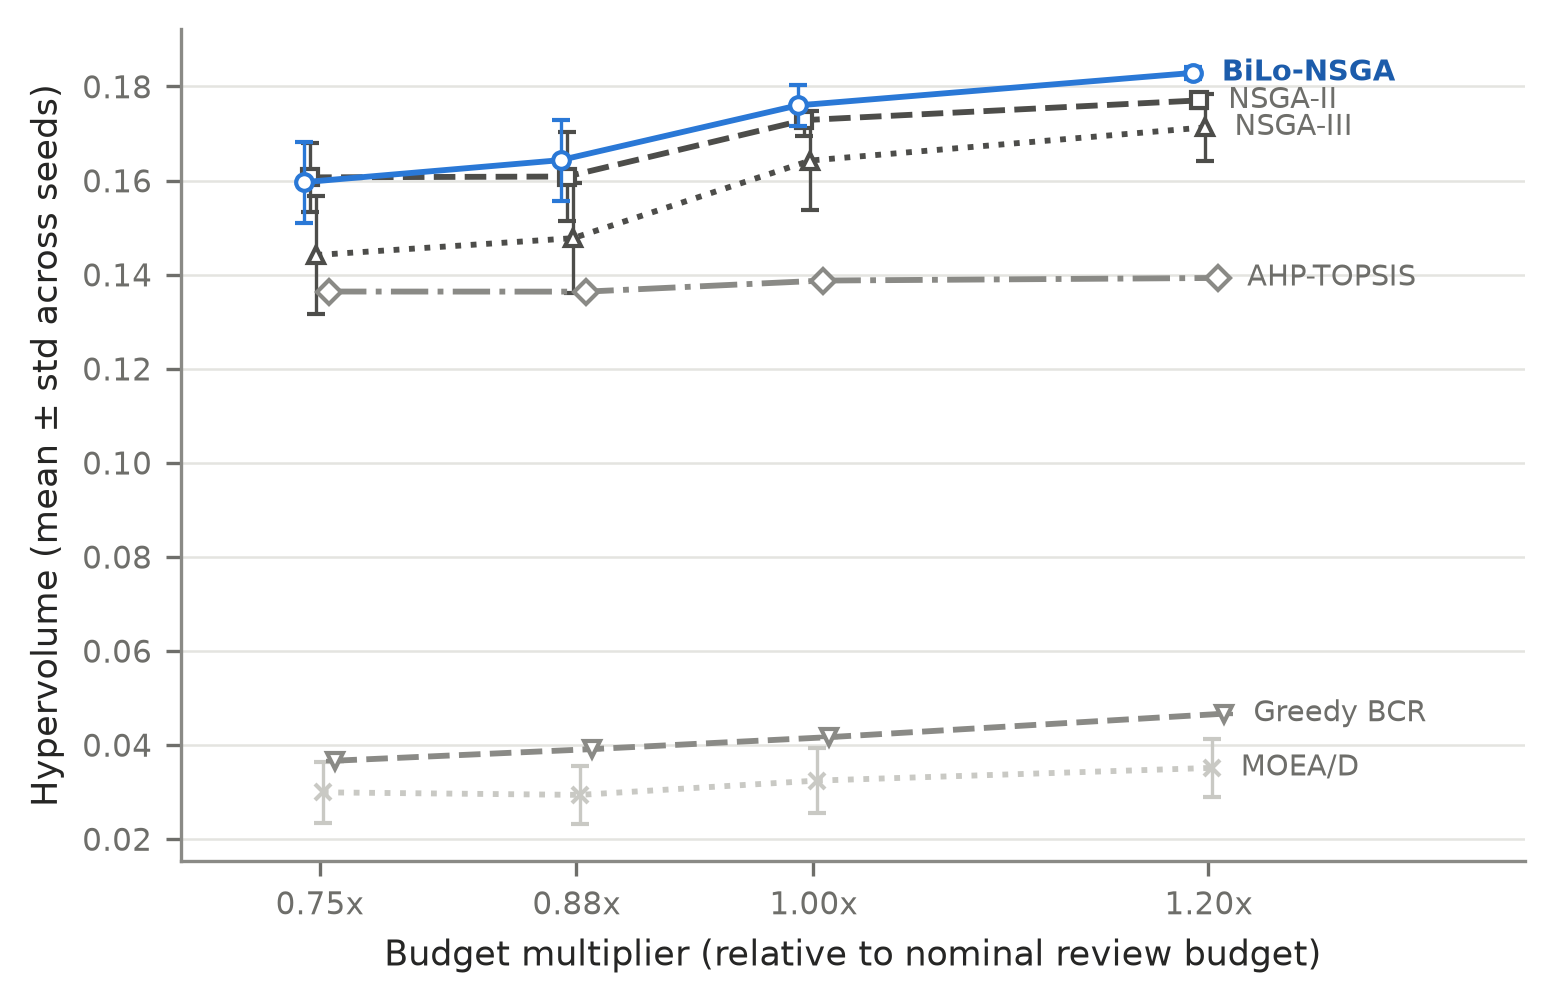
\includegraphics[width=0.94\textwidth]{figures/fig_budget_sensitivity.png}
\caption{Mean hypervolume (+- std across seeds) as a function of the budget multiplier for the six main methods; the two nominal-budget experiments are pooled at 1.00x.}\label{fig:3}
\end{figure*}

Mean hypervolume rises with the budget index for the principal methods. BiLo-NSGA's margin over NSGA-II ranges from -0.64\% at 0.75x and +2.17\% at 0.88x to +3.30\% in the 1.20x large-pool-labeled scenario. Because weights and seed streams are not held constant, this pattern cannot be attributed to budget headroom or forward insertion alone. The Ablation-LooseBudget stress rule, which searches at 1.2x and evaluates at the true constraint, is 6.35\% below the full method when pooled on this benchmark. This supports enforcing the declared budget during search in the tested setup, not a general monotone budget-regime claim.

\subsection{Ablation Study: Scenario-Dependent Forward Effects and Unresolved Substitution}\label{ablation-study-scenario-dependent-forward-effects-and-unresolved-substitution}

Figure 4 compares the full method with all ten ablations (pooled over 8 experiments x 30 seeds).

\begin{figure*}[t]
\centering

\includegraphics[width=0.94\textwidth]{figures/fig_ablation.png}
\caption{Mean hypervolume (+- std) of BiLo-NSGA and ten ablations or stress controls, pooled over all experiments and seeds. Formal decisions remain scenario-specific and Holm-adjusted.}\label{fig:4}
\end{figure*}

Removing evolution entirely reduces pooled hypervolume by 79.3\%. Disabling feasibility recovery costs 2.21\%, increases the standard deviation from 0.00861 to 0.01272, and lowers decision coverage from 0.996 to 0.928. By contrast, several local-operator ablations have pooled means above the full model. This prevents pooled ranking from being used as component attribution and makes the scenario-level tests essential.

\textbf{Forward insertion is the only local operator with resolved positive cells, but it is not universally beneficial.} Ablation-NoForwardSearch has pooled mean 0.17257, 0.39\% above the full method. Under the primary within-scenario family, the full method exceeds it in the dependency-constrained, local-move-explainability, and large-pool scenarios. An exploratory operator-specific Holm family across the eight scenarios also resolves reliability\_prioritized\_review (4/8), whereas the other four comparisons remain unresolved. The evidence therefore identifies scenario-dependent forward-side gains, not a pooled or universal benefit from insertion.

\textbf{Atomic substitution has no demonstrated accuracy gain.} Ablation-NoBackwardSearch reaches 0.17294, 0.61\% above the full method, and none of the eight differences is significant. The legacy standalone-deletion rule reaches 0.17228, 0.22\% above the full method, and is likewise inseparable in all eight scenarios. Feasibility recovery already removes weak projects after violations, leaving few replacements that improve the scalar acceptance score. The atomic rule is more faithful to project substitution, but the experiment supports its semantics, not its accuracy.

The substitution operator is retained because a single logged remove--insert pair is reviewable and cannot leave a deletion-only intermediate portfolio. A forward-only variant remains the evidence-supported lean implementation when that replacement semantic is unnecessary. Alternative acceptance based on dominance or bounded look-ahead is a redesign target, not part of the present claim.

Figure 5 separates move production from optimization quality. The new atomic substitution raises archive coverage relative to the no-backward variant but does not improve hypervolume at the available statistical resolution. Disabling forward search changes both event composition and scenario-level quality. These diagnostics do not imply that a larger move count is intrinsically better.

\begin{figure*}[t]
\centering
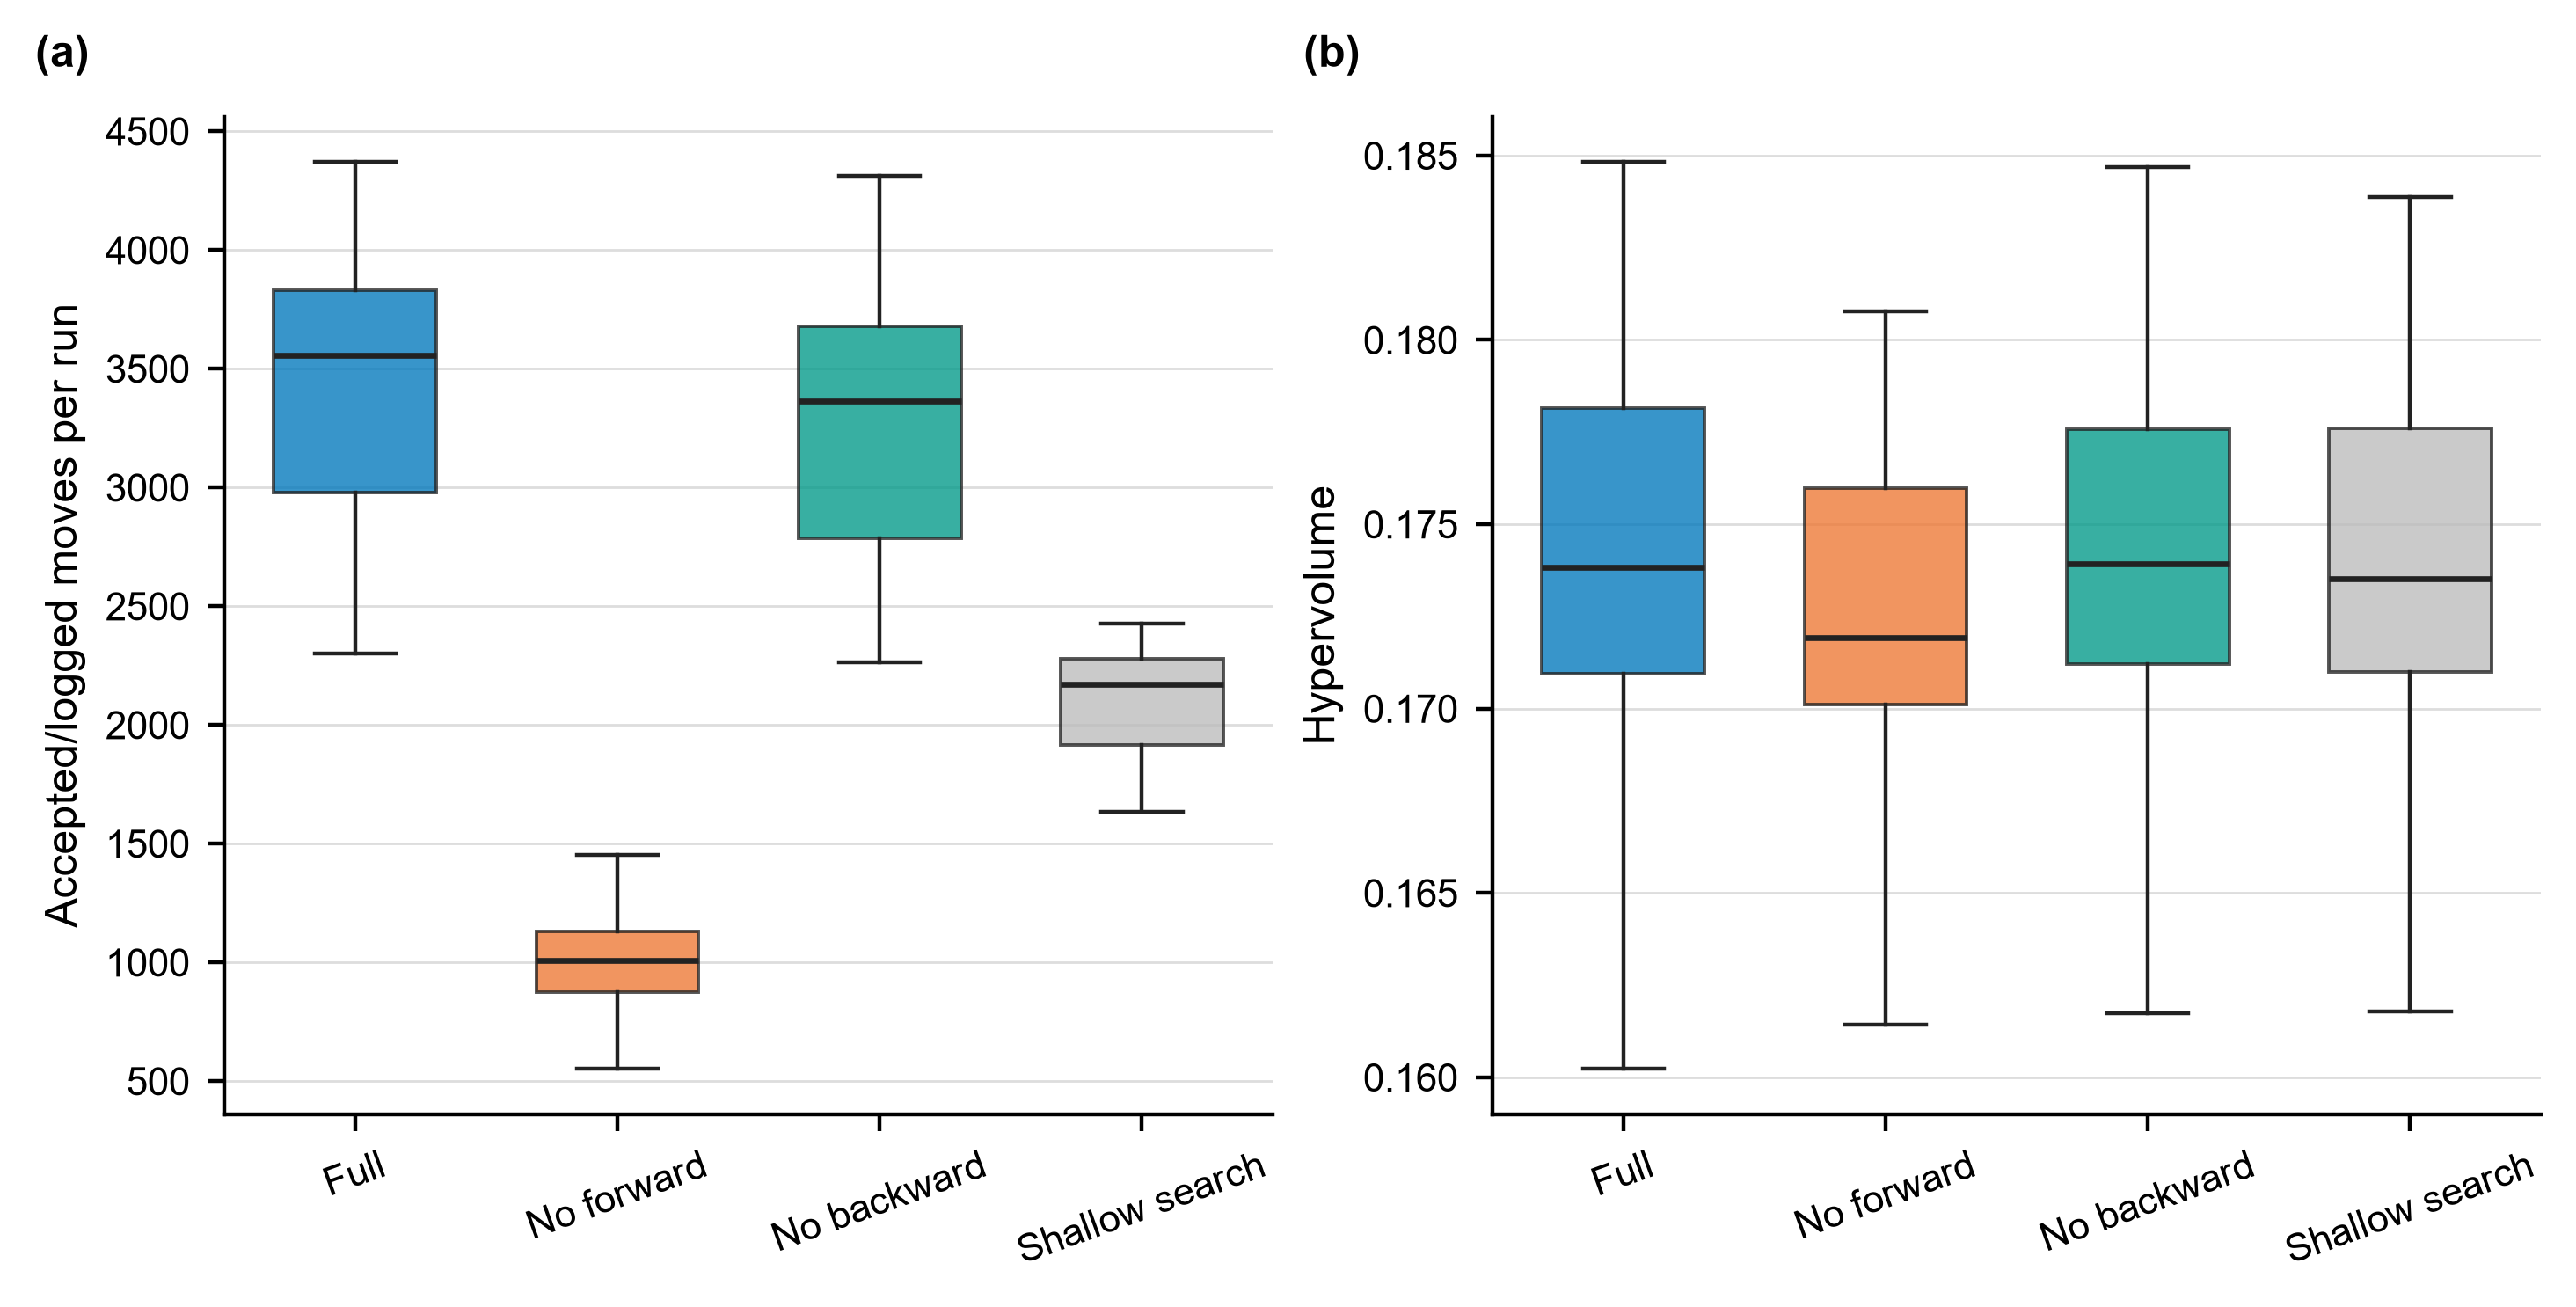
\includegraphics[width=0.94\textwidth]{figures/fig_move_diagnostics.png}
\caption{Local-search diagnostics pooled over eight experiments and 30 seeds (240 runs per configuration). (a) Logged accepted moves per run; (b) seed-level mean-front hypervolume. Boxes are descriptive aggregates. Formal component decisions use per-experiment Holm-adjusted tests.}\label{fig:5}
\end{figure*}

The two stress variants bound other claims. Thinning the dependency graph changes the pooled mean by less than 0.3\%, so no dependency-density gain is claimed. The LooseBudget variant's 6.35\% deficit was discussed in Section 6.2.

\subsection{External Consistency: NERC Rule-Based Backtest}\label{external-consistency-nerc-rule-based-backtest}

Hypervolume measures optimization quality on the benchmark objectives; it cannot show whether selected portfolios point at real risk. We therefore backtest selections against cached NERC reliability reports using a rule designed to reduce construct circularity. Each candidate receives a NERC-topic kind weight multiplied by a stress percentile computed from raw RTS/SimBench attributes before the NERC-based adjustment of Section 3.2. The priority-capture ratio measures oversampling of high-priority candidates relative to a uniform draw, with 1.0 denoting parity. Kendall's \(\tau\) measures rank alignment between selection frequency and priority. Figure 6 shows both review scenarios.

\begin{figure*}[t]
\centering
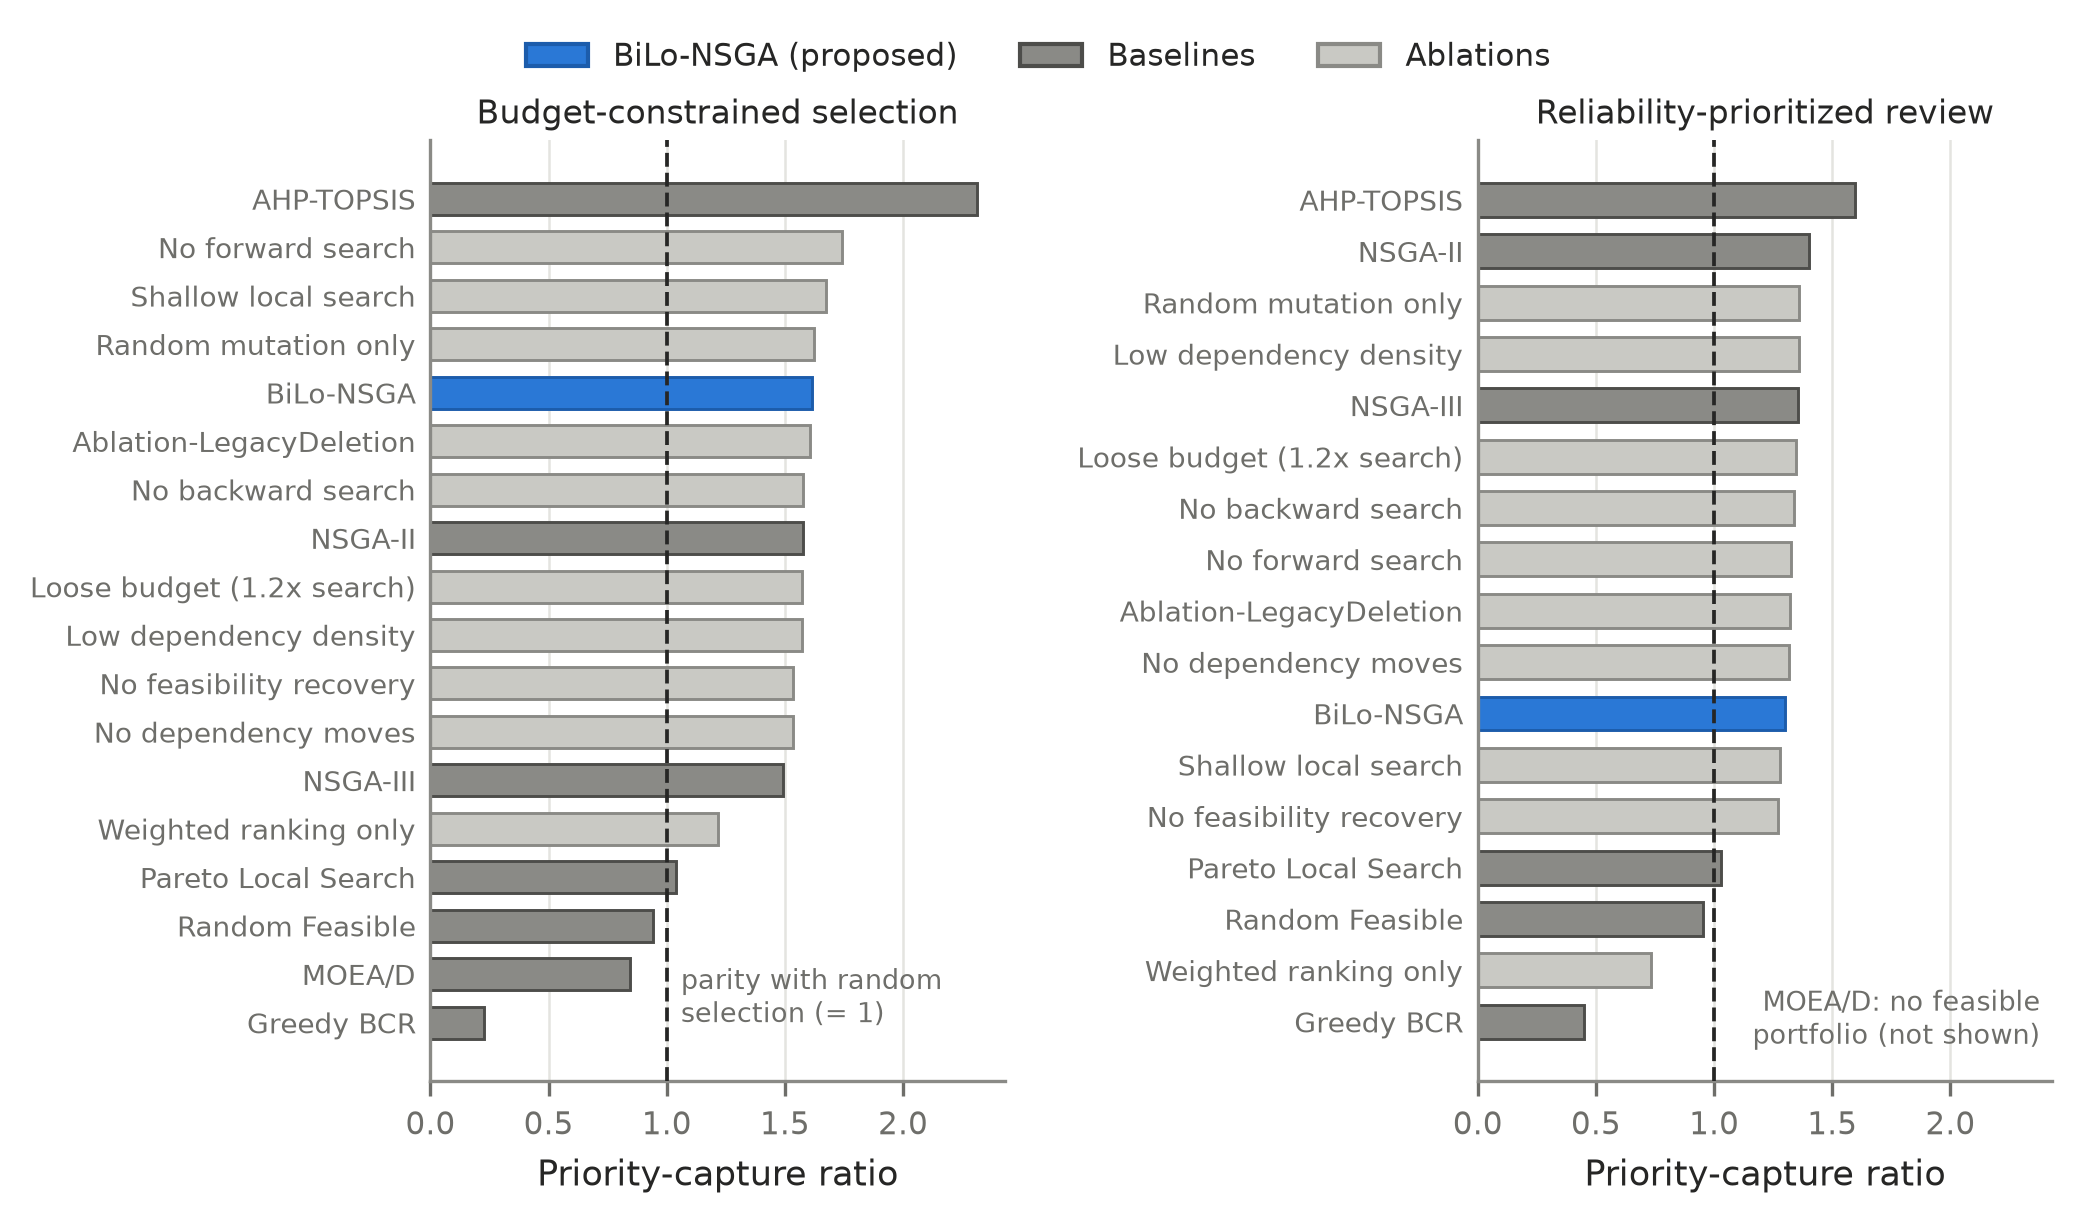
\includegraphics[width=0.94\textwidth]{figures/fig_nerc_backtest.png}
\caption{Priority-capture ratios in the NERC rule backtest (dashed line = parity with random selection). MOEA/D is absent from the reliability panel because it returned no feasible portfolio.}\label{fig:6}
\end{figure*}

BiLo-NSGA oversamples documented-risk candidates, with capture ratios of 1.617 in budget-constrained selection and 1.301 in reliability-prioritized review. These values are above NSGA-II in the first setting (1.575) and below it in the second (1.403). Kendall \(\tau\) values of 0.109 and 0.073 are not significant. AHP-TOPSIS has the highest nominal alignment because its reliability-type attributes overlap the rule. The backtest therefore indicates \textbf{descriptive external consistency only, not method superiority or ground-truth validity}. The stress-percentile component is independently derived, but kind-level weights retain construct overlap with pool generation.

\subsection{Historical Outcome Consistency: MISO MTEP16 Backtest}\label{historical-outcome-consistency-miso-mtep16-backtest}

The NERC backtest of Section 6.4 checks consistency against documented risk patterns from the same public corpus used in benchmark construction. A more independent check compares selections with \textbf{observed transmission-project outcomes} from the MISO MTEP16 Appendix A/B inventory. Outcome snapshots were not used in fitting. However, decision-time appendix status is a prognostic feature, creating construct overlap with the broad outcome definition.

\subsubsection{Data and Protocol}\label{data-and-protocol}

The MTEP16 dataset comprises 1218 projects with their 2016 cost estimates, project types, voltage levels, mileage, appendix status, and record dates. Quarterly Appendix A status snapshots from 2016-12 through 2018-01, together with the 2026 MISO portal in-service and active-project lists, produce three outcome classes:

\begin{itemize}
\tightlist
\item
  \textbf{Built} (n = 924): project ID appears in the 2026 in-service list or shows `In Service' in a snapshot.
\item
  \textbf{Withdrawn} (n = 19): explicitly withdrawn, never in service.
\item
  \textbf{Deferred} (n = 39): still active in the 2026 Appendix A, excluded from capture metrics.
\item
  \textbf{Unresolved} (n = 236): no trace in any 2026 list and never withdrawn; used only in the \emph{broad} negative definition.
\end{itemize}

For portability, each method selects compromise portfolios from 10 seeded runs, preserving 2016 cost estimates after one global scaling factor sets the flagship budget to 5\% of total pool cost. Point-biserial correlation and Mann--Whitney U compare selection frequency with broad or strict outcome labels; capture ratios relative to uniform selection are effect-size readouts. These are nominal project-level diagnostics. They do not preserve dependence among projects selected in the same portfolio, and no constrained-permutation or multiple-comparison family was preregistered. Two variants are shown: budget-constrained selection (1097 positive-cost projects) and reliability-prioritized review (1062 projects).

\subsubsection{Results}\label{results-1}

Table 6 summarizes the key comparisons.

\begin{table*}[t]
\centering
\scriptsize
\setlength{\tabcolsep}{3pt}
\caption{MTEP16 historical backtest in the budget-constrained experiment. P-values are nominal project-level diagnostics, not confirmatory portfolio-level tests.}\label{tab:6}
\begin{tabularx}{\textwidth}{@{}>{\raggedright\arraybackslash}X >{\raggedright\arraybackslash}X >{\raggedright\arraybackslash}X >{\raggedright\arraybackslash}X >{\raggedright\arraybackslash}X >{\raggedright\arraybackslash}X >{\raggedright\arraybackslash}X@{}}
\toprule
Method & Role & Capture (broad) & r\_pb (broad) & p (broad) & MW p (broad) & Portfolio size \\
\midrule
AHP-TOPSIS & baseline & 1.0995 & 0.128 & 0.00003 & 0.00003 & 320.0 \\
Ablation-NoFeasibilityRecovery & ablation & 1.0877 & 0.091 & 0.0031 & 0.0084 & 200.8 \\
Ablation-LowDependencyDensity & ablation & 1.0716 & 0.089 & 0.0037 & 0.0173 & 247.0 \\
\textbf{BiLo-NSGA} & \textbf{proposed} & \textbf{1.0715} & \textbf{0.088} & \textbf{0.0042} & \textbf{0.0147} & \textbf{243.0} \\
Pareto Local Search & baseline & 1.0343 & 0.049 & 0.109 & 0.067 & 166.2 \\
NSGA-III & baseline & 1.0283 & 0.050 & 0.101 & 0.090 & 110.1 \\
Greedy BCR & baseline & 1.0267 & 0.057 & 0.062 & 0.062 & 585.0 \\
NSGA-II & baseline & 1.0118 & 0.025 & 0.425 & 0.264 & 124.7 \\
Random Feasible & baseline & 0.9893 & -0.019 & 0.534 & 0.686 & 93.0 \\
\bottomrule
\end{tabularx}
\end{table*}

BiLo-NSGA's broad capture is 1.071, or 7.1\% above the numerical uniform-draw reference. The raw diagnostics are point-biserial \(r=0.088\) (\(p=0.0042\)) and Mann--Whitney \(p=0.0147\). It exceeds the tested evolutionary and local-search baselines on broad capture, including Pareto Local Search at 1.034 and NSGA-II at 1.012, but AHP-TOPSIS is higher at 1.100. NoFeasibilityRecovery reaches 1.088 and LowDependencyDensity 1.072. The reliability-prioritized variant is directionally similar (capture 1.064, \(r=0.078\), raw \(p=0.0128\)). These descriptive results do not identify a local operator or establish portfolio-level significance.

\textbf{AHP-TOPSIS achieves the highest nominal broad capture (1.100)} because it directly optimizes evidence/compliance features that overlap Appendix-status information. Within the strict built-versus-withdrawn subset, BiLo-NSGA's capture is 1.009; MOEA/D and NSGA-II are nominally higher at 1.011 and 1.010. We therefore present the rerun as a \textbf{descriptive external-consistency result}. Strict labels remain underpowered, alternative ablations can align more strongly, and no superiority claim is made.

\subsubsection{Outcome-Definition and Dependence Limits}\label{outcome-definition-and-dependence-limits}

We state the caveats that limit the strength of this backtest.

\begin{itemize}
\tightlist
\item
  \textbf{Base-rate ceiling.} MTEP16 Appendix A projects were overwhelmingly built (\textasciitilde98\% within the strict subset). MTEP board approval itself is a strong filter; this backtest measures alignment \emph{within} an already-approved plan, not the value of the review filter itself.
\item
  \textbf{Low strict power.} With only 19 explicit withdrawals, the strict-label Mann-Whitney and point-biserial tests are low-powered, and a null result is expected even for a well-aligned method. The broad view has more negative instances (withdrawn + unresolved) but the \texttt{unresolved} class may include projects rebuilt under new MTEP IDs.
\item
  \textbf{Type-distribution shift.} The real MTEP16 pool is dominated by reliability, asset-condition, and distribution projects; renewable and storage projects are nearly absent. The pipeline's renewable objective is therefore close to inert in this backtest, and renewable-related claims receive no support from this rung.
\item
  \textbf{Appendix status as feature.} The \texttt{appendix\_status} attribute (A / B-to-A / B) is used as an evidence feature. This is decision-time information (2016 board approval state), not an outcome, but it correlates with broad outcomes. Broad capture partly rewards methods that weight evidence/compliance features, which is why AHP-TOPSIS excels; strict capture (within board-approved Appendix A projects) is the cleaner discriminator.
\item
  \textbf{Protocol differences.} Unlike the main experiments (30 seeds, hypervolume evaluation), the MTEP backtest uses 10 seeded runs and compromise-portfolio selection to align with real portfolio sizes. Point-biserial and Mann-Whitney are the primary readouts; capture ratios are effect-size indicators given the ceiling constraints.
\end{itemize}

\subsection{Search-Effort and Outcome-Definition Diagnostics}\label{search-effort-and-outcome-definition-diagnostics}

The method's pooled gain over NSGA-II is modest, so computation and trace production are shown beside hypervolume. BiLo-NSGA averages 0.17190 hypervolume, 0.2188 s, 3668 accepted local-search events, and 0.996 decision coverage. NSGA-II averages 0.17000 at 0.0798 s and emits no move trace. Thus, the 1.12\% pooled hypervolume margin costs a 2.74-fold runtime factor in the tested implementation, while the trace is an additional decision-support output rather than free metadata.

\begin{figure*}[t]
\centering

\includegraphics[width=0.94\textwidth]{figures/fig_search_audit_efficiency.png}
\caption{Pooled search-and-trace diagnostics over eight experiments and 30 seeds. Each panel retains its native unit; no composite score is formed from optimization quality and trace volume.}\label{fig:7}
\end{figure*}

\begin{table*}[t]
\centering
\scriptsize
\setlength{\tabcolsep}{3pt}
\caption{Selected pooled quality--effort readouts.}\label{tab:7}
\begin{tabularx}{\textwidth}{@{}>{\raggedright\arraybackslash}X >{\raggedright\arraybackslash}X >{\raggedright\arraybackslash}X >{\raggedright\arraybackslash}X >{\raggedright\arraybackslash}X >{\raggedright\arraybackslash}X@{}}
\toprule
Method & Mean HV & Runtime (s) & Accepted/logged moves & Coverage & Evidence implication \\
\midrule
BiLo-NSGA & 0.17190 & 0.2188 & 3668.0 & 0.996 & forward insertion plus atomic substitution \\
NoBackwardSearch & 0.17294 & 0.1616 & 3295.2 & 0.978 & nominally higher HV; no significant difference \\
LegacyDeletion & 0.17228 & 0.1933 & 3438.6 & 0.984 & atomic and legacy rules are inseparable \\
NoForwardSearch & 0.17257 & 0.1139 & 1563.6 & 0.999 & higher pooled HV; full wins significantly in 3/8 scenarios \\
NSGA-II & 0.17000 & 0.0798 & 0 & --- & strongest external evolutionary baseline \\
AHP-TOPSIS & 0.13875 & 0.0004 & 0 & --- & very low cost, lower proxy-objective coverage \\
\bottomrule
\end{tabularx}
\end{table*}

Table 7 makes the operator evidence operational. Removing atomic substitution reduces runtime by about 26\% and nominally raises hypervolume by 0.61\%, with the contrast unresolved under the declared comparison family. The contrast with standalone deletion also remains unresolved. Removing forward search lowers runtime and raises the pooled mean, but the full method wins significantly in three named scenarios. A forward-only variant is therefore the lean configuration; the full version is justified when a review process requires atomic replacement records.

Figure 8 exposes outcome-definition sensitivity. BiLo-NSGA's broad capture is 1.0715 and 1.0642 across the two scenarios, whereas strict capture is 1.0093 and 1.0042. Raw broad correlations are nonzero under conventional project-level tests, but broad negatives include unresolved projects and portfolio dependence is unmodeled. The strict comparison is less ambiguous, yet contains only 19 withdrawals and has little power.

\begin{figure*}[t]
\centering

\includegraphics[width=0.94\textwidth]{figures/fig_mtep_outcome_backtest.png}
\caption{MTEP16 outcome-capture ratios for the proposed method and baselines. The dashed line denotes parity with uniform selection. Broad and strict labels are shown separately so that the high built-project base rate and unresolved-project assumption remain visible.}\label{fig:8}
\end{figure*}

These diagnostics assemble two decision-relevant views: optimization gain per unit of search and trace production, and outcome consistency under competing label definitions. BiLo-NSGA improves the tested front modestly and produces dense move histories, but atomic substitution is not supported as an accuracy mechanism and the historical backtest remains descriptive.

\subsection{Direct Local-Search and Substitution Controls}\label{direct-local-search-and-substitution-controls}

Pareto Local Search supplies a direct non-evolutionary neighborhood-search baseline with add, delete, and swap moves under 1600 evaluated neighbors per run. Its pooled hypervolume is 0.11636, compared with 0.17190 for BiLo-NSGA, and the proposed method is significantly higher in all eight scenarios after Holm correction. The numerical evaluation ceilings are matched, but computational work is not identical; PLS is slower in this implementation (1.416 s per run). The finding therefore applies to the disclosed PLS configuration rather than to Pareto local search as a family.

Figure 9 places that baseline beside the three operator controls. NoBackwardSearch (0.17294) and LegacyDeletion (0.17228) both have higher pooled means than the atomic full method, although no scenario-level comparison is significant. NoForwardSearch (0.17257) also has a higher pooled mean, while the full method has three significant scenario wins. The figure therefore closes a comparator gap without creating a bidirectional-gain claim.

\begin{figure*}[t]
\centering
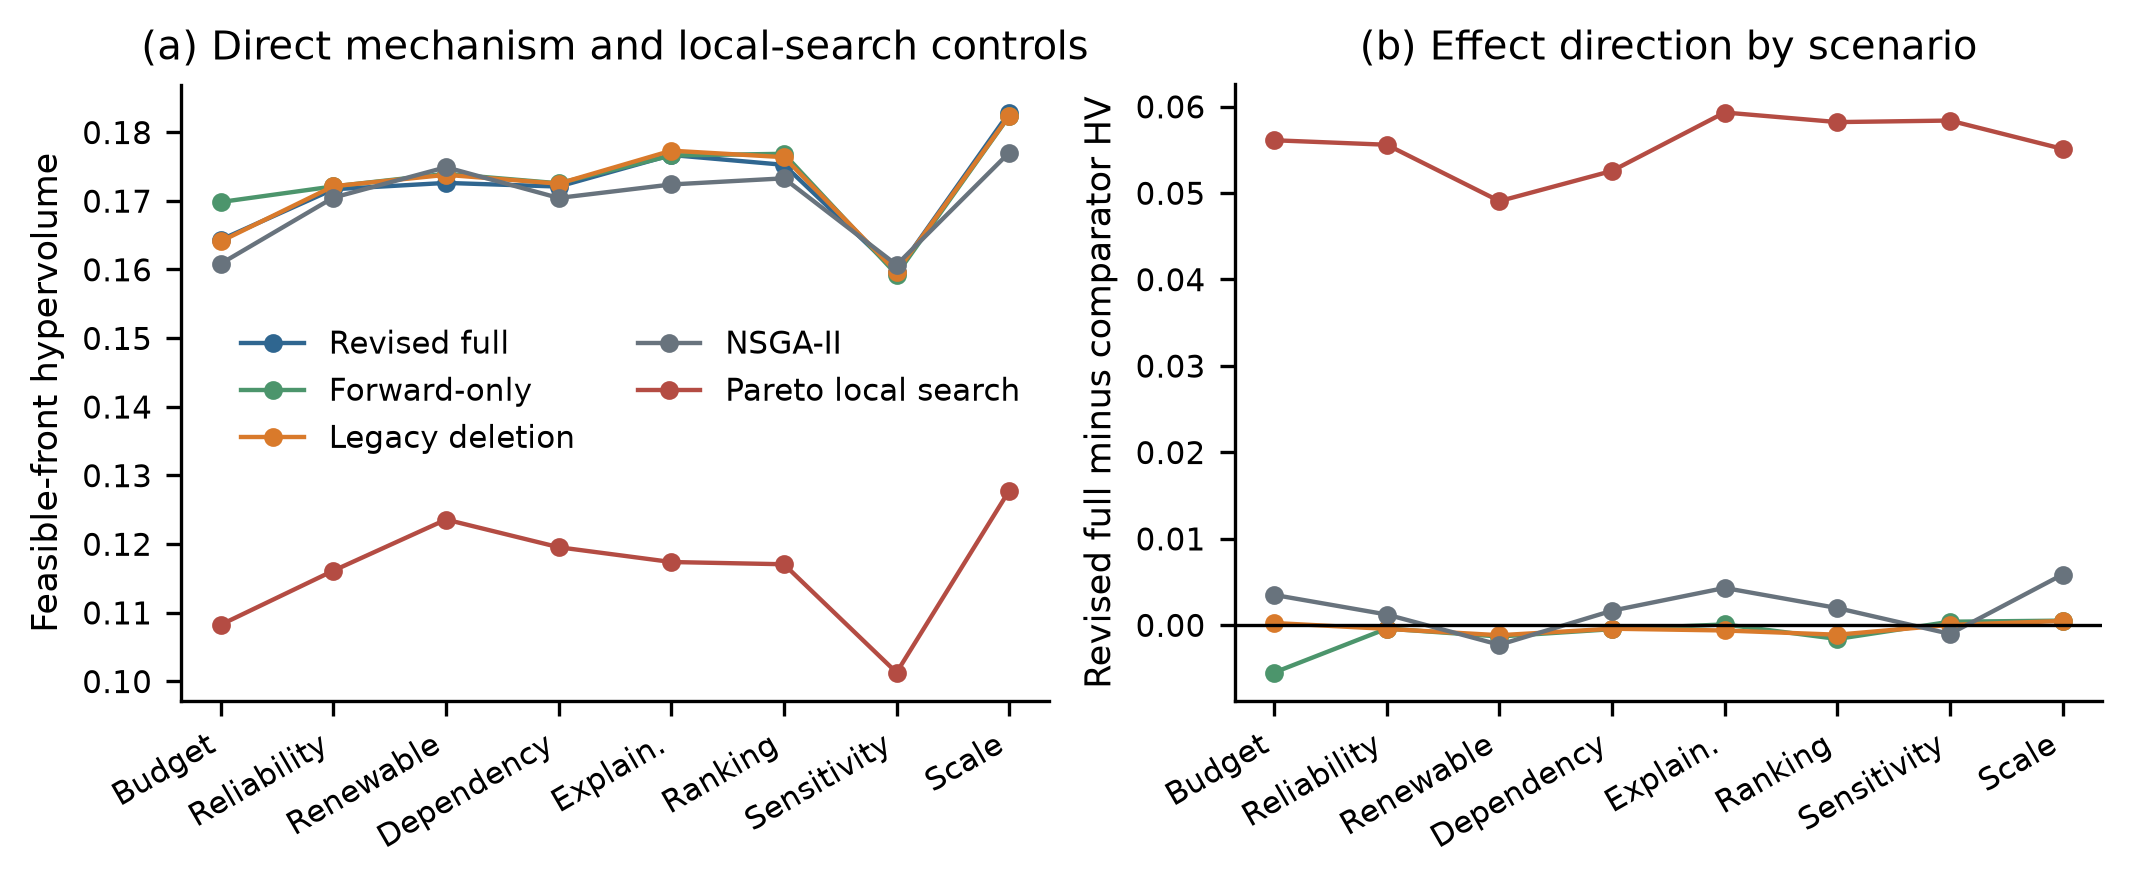
\includegraphics[width=0.94\textwidth]{figures/fig_atomic_substitution_controls.png}
\caption{Pooled hypervolume and scenario-level significance counts for BiLo-NSGA, Pareto Local Search, NoForwardSearch, NoBackwardSearch, and LegacyDeletion. The direct PLS control is separated in all eight scenarios; the three operator controls delimit the mechanism claim.}\label{fig:9}
\end{figure*}

\begin{center}\rule{0.5\linewidth}{0.5pt}\end{center}

\section{Discussion}\label{discussion}

\textbf{Why the resolved operator effects are forward-side.} Under deterministic repair, populations remain near the budget boundary. Forward insertion can exploit residual slack directly. Atomic substitution must find a removal, an affordable replacement, and a joint scalar improvement in one step, while repair has already removed many weak projects. This makes substitution opportunities rarer, but the explanation remains an inference from the observed event and ablation patterns rather than a proved mechanism.

The operator effects depend on the scenario. The no-forward ablation has a higher pooled mean, yet the full method wins significantly in three scenarios; no corresponding significant gain exists for atomic substitution. The full substitution rule is retained for reviewable replacement semantics. A look-ahead or dominance-based acceptance rule is the appropriate redesign target.

\textbf{What the external-consistency checks add.} The NERC rule check (Section 6.4) shows concentration on documented risk patterns but retains construct overlap with pool generation. The MTEP16 backtest (Section 6.5) uses independent historical outcomes and 2016-vintage features, but its project-level diagnostics ignore portfolio dependence and face a severe outcome base rate. Together, they test whether optimized portfolios immediately contradict two public-record views; they do not replace expert-labeled feasibility outcomes or calibrated costs.

\textbf{Positioning against TRACE-MOEA.} The companion study {[}33{]} uses a preference-adaptive ranking layer, repair, and a trace archive over the same public candidate pipeline. BiLo-NSGA instead studies project-vocabulary variation under a hard budget. Its central questions concern forward insertion, atomic substitution, and the 6.35\% cost of budget-blind search. The methods share candidate generation but not their core operators, scenario design, or analyses.

\textbf{Practical implications.} The method's NSGA-II margin ranges from -0.64\% at 0.75x to +3.30\% at 1.20x, with a 2.74x runtime factor; all evolutionary runs remain sub-second. A forward-only implementation is defensible where the review process does not require atomic replacement records. Pareto Local Search is a useful direct comparator but is substantially weaker and slower under the matched neighbor budget.

The recorded move history covers 99.6\% of projects in the returned fronts with at least one operation, but explanation sufficiency has not been validated with human evaluators. If single-criterion regulatory alignment is dominant, AHP-TOPSIS remains competitive. The MTEP16 backtest supplies only weak-form evidence that BiLo-NSGA selections correlate with real outcomes.

\subsection{Evidence-Driven Extensions}\label{evidence-driven-extensions}

The results identify five empirical extensions that would test the framework beyond its current proxy setting.

\begin{enumerate}
\def\labelenumi{\arabic{enumi}.}
\tightlist
\item
  \emph{Proxy review task without expert labels} (Limitation 1). Next step: recruit a small panel of utility planning engineers to independently rank a stratified subset of the 120 candidates, and report the rank correlation between expert priorities and the benchmark's derived attributes; this converts the proxy claim into a measurable calibration statement.
\item
  \emph{Costs not monetarily calibrated} (Limitation 2). Next step: fit the synthetic cost units against published per-category investment figures -- the MISO MTEP cost estimates already cached for the Section 6.5 backtest are a natural anchor -- and re-run the flagship budget-constrained scenario with calibrated coefficients to test whether the method ordering is preserved.
\item
  \emph{External validity below the expert-label rung} (Limitation 3). Next step: extend the MTEP backtest to later plan cohorts (MTEP17--MTEP19), which multiplies the number of explicitly withdrawn projects beyond the current n = 19 and gives the strict-label tests the statistical power they presently lack.
\item
  \emph{Single benchmark family} (Limitation 4). Next step: instantiate a second candidate pool from an independent public system (NREL-118 or a TAMU synthetic case) through the released derivation pipeline; two scenarios with the main baseline comparison suffice to test whether the forward/substitution asymmetry and the budget-margin pattern generalize.
\item
  \emph{No load-flow verification} (Limitation 5). Next step: run a pandapower AC load-flow check on the compromise portfolios of the two reliability-oriented scenarios and report electrical-violation rates, upgrading portfolio feasibility from budgetary to physical.
\end{enumerate}

The ablation evidence motivates a method redesign. Future atomic substitution should test bounded look-ahead or dominance-based acceptance (Section 6.3). A sensitivity analysis of scalarization weights and the dependency bonus would also characterize two remaining default hyperparameters.

\begin{center}\rule{0.5\linewidth}{0.5pt}\end{center}

\section{Limitations}\label{limitations}

We state the boundaries of this study explicitly.

\begin{enumerate}
\def\labelenumi{\arabic{enumi}.}
\item
  \textbf{Proxy review task without expert labels.} The 120 candidates and their attributes are derived from public grid statistics and reliability-report metadata through published rules; no expert-labeled review outcomes exist in the benchmark. All claims are therefore claims about \emph{algorithmic performance on a reproducible public proxy}, not about validated real-world review quality. Expert-labeled subsets (with rank-correlation analysis against the proxy) are the direct remedy.
\item
  \textbf{Costs are not monetarily calibrated.} Candidate costs are synthetic cost units generated from network aggregates. Calibrating coefficients against published utility investment figures is required before any engineering-economic claim.
\item
  \textbf{External checks do not reach the expert-label rung.} The NERC rule backtest retains kind-level construct overlap with pool generation. MTEP16 outcome snapshots were not used in fitting, but decision-time appendix status is prognostic and the project-level tests do not preserve portfolio dependence or a multiplicity family. The approved-plan pool also has an approximately 98\% strict-label build rate and almost no renewable projects. These checks are descriptive consistency evidence.
\item
  \textbf{Single benchmark family.} All eight scenarios instantiate one 120-candidate pool from one RTS-GMLC + SimBench + NERC derivation. A second pool from independent public systems would test whether the forward/substitution asymmetry and the budget-margin pattern generalize.
\item
  \textbf{No load-flow verification.} Portfolio feasibility is budgetary, not electrical; a pandapower-based load-flow check of selected portfolios is a natural robustness addition.
\item
  \textbf{The direct local-search comparison is still bounded.} Pareto Local Search adds a matched-budget add/delete/swap neighborhood baseline, and BiLo-NSGA significantly exceeds it in all eight scenarios. However, this is one implementation and does not cover the full family of memetic, large-neighborhood, or exact knapsack algorithms. No universal local-search superiority claim is made.
\end{enumerate}

\begin{center}\rule{0.5\linewidth}{0.5pt}\end{center}

\section{Conclusions}\label{conclusions}

BiLo-NSGA defines local-search moves in project-review terms: insertion under slack, atomic delete--insert substitution, dependency-aware bonuses, feasibility recovery, and per-move logging. On the 120-candidate public proxy benchmark, it improves pooled hypervolume over NSGA-II by 1.12\%. Across five stochastic baselines, it records 36 significant wins among 40 comparisons and no significant loss; 16 deterministic-rule gaps are descriptive and favor BiLo-NSGA. Pareto Local Search is significantly lower in all eight scenarios. The NSGA-II margin ranges from -1.31\% to +3.30\% across settings.

The component result is asymmetric. Under the primary within-scenario family, removing forward insertion is significantly harmful in three scenarios but raises the pooled mean. Removing atomic substitution raises the pooled mean by 0.61\%, and the contrasts involving atomic substitution and legacy deletion remain unresolved under the declared comparison family. Forward insertion therefore produces the only resolved local-operator gains. Atomic substitution remains useful as a single recorded replacement operation, but its acceptance rule requires redesign before it can be presented as a performance mechanism; move-history statistics never enter optimization ranking.

The NERC and MTEP16 backtests provide descriptive external consistency. MTEP16 broad capture is 1.071 and the raw point-biserial association is 0.088; strict-label ordering is unresolved. The study consequently supports BiLo-NSGA as a project-level local-search framework on the public proxy benchmark, with forward-only search as the lean configuration when atomic replacement records are unnecessary. Expert labels, calibrated costs, a second benchmark family, broader local-search comparisons, and load-flow verification remain necessary to evaluate practical review effectiveness.

\begin{center}\rule{0.5\linewidth}{0.5pt}\end{center}

\section*{Author Contributions}

{[}AUTHOR INPUT REQUIRED: assign the CRediT roles to Yubin Lin, Jingbo Zhang, Xiaoyu Huang, Dishan Yang, and Jiyu Li, and obtain approval from every author.{]} All authors have read and agreed to the published version of the manuscript.

\section*{Funding}

{[}AUTHOR INPUT REQUIRED: insert the verified funder, grant number, and APC funder, or state ``This research received no external funding.''{]}

\section*{Institutional Review Board Statement}

Not applicable.

\section*{Informed Consent Statement}

Not applicable.

\section*{Data Availability Statement}

All data used in this study are public. Candidate projects are derived from RTS-GMLC (https://github.com/GridMod/RTS-GMLC), SimBench (https://simbench.de), and metadata from public NERC reliability reports (https://www.nerc.com). MISO MTEP16 records are available through the MISO transmission-planning archive (https://www.misoenergy.org/planning/transmission-planning). The candidate pipeline, BiLo-NSGA implementation, configurations, 4320 per-run records, corrected inference tables, backtest data, and figure scripts are included in the supplementary review package and are available from the corresponding author. Pre-atomic-substitution backtests remain explicitly suffixed and excluded. A persistent public archive can be supplied before publication, subject to third-party redistribution terms. TRACE-MOEA shares the versioned candidate generator, NERC source corpus, and public MTEP16 records. Problem objectives, algorithm implementations, scenarios, run archives, selected portfolios, and reported comparisons are paper-specific.

\section*{Acknowledgments}

During the preparation of this manuscript, the authors used Claude (Anthropic) for language refinement, literature summary, and formatting assistance under the authors' full intellectual oversight. The authors reviewed and revised all assisted content and take full responsibility for the publication.

\section*{Conflicts of Interest}

The authors declare no conflicts of interest.

\begin{center}\rule{0.5\linewidth}{0.5pt}\end{center}

\begin{thebibliography}{99}
\bibitem{ref1} Zitzler, E.; Thiele, L. Multiobjective evolutionary algorithms: a comparative case study and the strength Pareto approach. \emph{IEEE Transactions on Evolutionary Computation} 1999, 3(4), 257--271. \url{https://doi.org/10.1109/4235.797969}
\bibitem{ref2} Jaszkiewicz, A. Genetic local search for multi-objective combinatorial optimization. \emph{European Journal of Operational Research} 2002, 137(1), 50--71. \url{https://doi.org/10.1016/S0377-2217(01})00104-7
\bibitem{ref3} Lust, T.; Teghem, J. The multiobjective multidimensional knapsack problem: a survey and a new approach. \emph{International Transactions in Operational Research} 2012, 19(4), 495--520. \url{https://doi.org/10.1111/j.1475-3995.2011.00840.x}
\bibitem{ref4} Feng, Y.; Hu, T.; Chen, X.-A.; Wang, G.-G. Recent Advances in Knapsack Problem: A Comprehensive Review of Models, Algorithms, and Applications. \emph{Neurocomputing} 2026, 666, 132135. \url{https://doi.org/10.1016/j.neucom.2025.132135}
\bibitem{ref5} Ishibuchi, H.; Akedo, N.; Nojima, Y. Behavior of Multiobjective Evolutionary Algorithms on Many-Objective Knapsack Problems. \emph{IEEE Transactions on Evolutionary Computation} 2015, 19(2), 264--283. \url{https://doi.org/10.1109/TEVC.2014.2315442}
\bibitem{ref6} Doerner, K.; Gutjahr, W.J.; Hartl, R.F.; Strauss, C.; Stummer, C. Pareto Ant Colony Optimization: A Metaheuristic Approach to Multiobjective Portfolio Selection. \emph{Annals of Operations Research} 2004, 131(1--4), 79--99. \url{https://doi.org/10.1023/B:ANOR.0000039513.99038.c6}
\bibitem{ref7} Carazo, A.F.; Gomez, T.; Molina, J.; Hernandez-Diaz, A.G.; Guerrero, F.M.; Caballero, R. Solving a comprehensive model for multiobjective project portfolio selection. \emph{Computers \& Operations Research} 2010, 37(4), 630--639. \url{https://doi.org/10.1016/j.cor.2009.06.012}
\bibitem{ref8} Gao, C.; Wang, X.; Li, D.; Han, C.; You, W.; Zhao, Y. A Novel Hybrid Power-Grid Investment Optimization Model with Collaborative Consideration of Risk and Benefit. \emph{Energies} 2023, 16(20), 7215. \url{https://doi.org/10.3390/en16207215}
\bibitem{ref9} Xiong, H.; Feng, B.; Yan, F.; Kang, Y.; Hu, Y.; Li, Q.; Tan, Q. A Hybrid Heuristic-Benders Method for Wind-Hydrogen Investment Planning with Non-Analytical Cost Functions. \emph{Energies} 2026, 19(9), 2172. \url{https://doi.org/10.3390/en19092172}
\bibitem{ref10} Liang, Y.; Liu, H.; Zhou, H.; Meng, Z.; Liu, J.; Zhou, M. Multi-Stage Coordinated Planning for Transmission and Energy Storage Considering Large-Scale Renewable Energy Integration. \emph{Applied Sciences} 2024, 14(15), 6486. \url{https://doi.org/10.3390/app14156486}
\bibitem{ref11} Bhattarai, S.; Karki, R. Interruption Cost Estimation for Value-Based Reliability Investment in Emerging Smart Grid Resources. \emph{Applied Sciences} 2024, 14(19), 8651. \url{https://doi.org/10.3390/app14198651}
\bibitem{ref12} Zhang, T.; Wu, J.; Hong, J.; Zhou, H.; Zheng, J.; Zheng, Z.; Niu, C.; Gao, Z.; Peng, L.; Lin, Z. Optimal Planning and Investment Return Analysis of Grid-Side Energy Storage System Addressing Multi-Dimensional Grid Security Requirements. \emph{Applied Sciences} 2025, 15(22), 11944. \url{https://doi.org/10.3390/app152211944}
\bibitem{ref13} Shen, F.; Luo, Q. A Multi-Objective Optimization Framework for Optimal Configuration of Battery Energy Storage System in Peak Shaving and Valley Filling Scenarios. \emph{Applied Sciences} 2026, 16(5), 2357. \url{https://doi.org/10.3390/app16052357}
\bibitem{ref14} Saaty, T.L. \emph{The Analytic Hierarchy Process: Planning, Priority Setting, Resource Allocation}; McGraw-Hill: New York, NY, USA, 1980.
\bibitem{ref15} Hwang, C.-L.; Yoon, K. \emph{Multiple Attribute Decision Making: Methods and Applications}. Lecture Notes in Economics and Mathematical Systems, Vol. 186; Springer: Berlin/Heidelberg, Germany, 1981.
\bibitem{ref16} Mizrak, F.; Yasar, O. A Secondary-Data-Driven Decision Support Framework for Strategic Energy Investment Prioritization: An Explainable Multi-Criteria Application Across Countries. \emph{Energies} 2026, 19(14), 3243. \url{https://doi.org/10.3390/en19143243}
\bibitem{ref17} Yang, L.; Zhao, S.; Gao, P.; Feng, X.; Guo, C. A Review of Multi-Objective Optimization-Based Site Selection for Power Plants: Principles and Methods. \emph{Applied Sciences} 2026, 16(13), 6727. \url{https://doi.org/10.3390/app16136727}
\bibitem{ref18} Lu, X.; Li, F.; Liu, J.; Yang, C.; Lin, L. Quantitative Evaluation of Crucial Substations and Simulation-Driven Impact Assessment of Commissioning Delays in Multi-Voltage Grid Planning. \emph{Electronics} 2025, 14(13), 2633. \url{https://doi.org/10.3390/electronics14132633}
\bibitem{ref19} Wu, Q.; Zhou, M.; Yan, J.; Sang, Z.; Wang, S. A survey on investment efficiency-oriented power grid infrastructure planning. \emph{Frontiers in Energy Research} 2025, 13, 1561763. \url{https://doi.org/10.3389/fenrg.2025.1561763}
\bibitem{ref20} Ishibuchi, H.; Murata, T. A multi-objective genetic local search algorithm and its application to flowshop scheduling. \emph{IEEE Transactions on Systems, Man, and Cybernetics, Part C} 1998, 28(3), 392--403. \url{https://doi.org/10.1109/5326.704576}
\bibitem{ref21} Knowles, J.D.; Corne, D.W. Approximating the Nondominated Front Using the Pareto Archived Evolution Strategy. \emph{Evolutionary Computation} 2000, 8(2), 149--172. \url{https://doi.org/10.1162/106365600568167}
\bibitem{ref22} Deb, K.; Pratap, A.; Agarwal, S.; Meyarivan, T. A fast and elitist multiobjective genetic algorithm: NSGA-II. \emph{IEEE Transactions on Evolutionary Computation} 2002, 6(2), 182--197. \url{https://doi.org/10.1109/4235.996017}
\bibitem{ref23} Zhang, Q.; Li, H. MOEA/D: A Multiobjective Evolutionary Algorithm Based on Decomposition. \emph{IEEE Transactions on Evolutionary Computation} 2007, 11(6), 712--731. \url{https://doi.org/10.1109/TEVC.2007.892759}
\bibitem{ref24} Deb, K.; Jain, H. An Evolutionary Many-Objective Optimization Algorithm Using Reference-Point-Based Nondominated Sorting Approach, Part I: Solving Problems With Box Constraints. \emph{IEEE Transactions on Evolutionary Computation} 2014, 18(4), 577--601. \url{https://doi.org/10.1109/TEVC.2013.2281535}
\bibitem{ref25} Neri, F.; Cotta, C. Memetic algorithms and memetic computing optimization: A literature review. \emph{Swarm and Evolutionary Computation} 2012, 2, 1--14. \url{https://doi.org/10.1016/j.swevo.2011.11.003}
\bibitem{ref26} He, R.; Hao, J.; Zhou, H.; Chen, F. Multi-Objective Collaborative Optimization of Distribution Networks with Energy Storage and Electric Vehicles Using an Improved NSGA-II Algorithm. \emph{Energies} 2025, 18(19), 5232. \url{https://doi.org/10.3390/en18195232}
\bibitem{ref27} Lin, X.; Meng, W.; Yu, M.; Yang, Z.; Luo, Q.; Rao, Z.; Peng, J.; Chen, Y. Multi-Objective Optimization of Offshore Wind Farm Configuration for Energy Storage Based on NSGA-II. \emph{Energies} 2025, 18(12), 3061. \url{https://doi.org/10.3390/en18123061}
\bibitem{ref28} Ding, J.; Liao, Q.; Tang, F.; Li, B.; Yu, Y.; Zhou, T. Bi-Objective Resilient Backbone-Grid Planning via a Three-Stage TER-NSGA-II Approach Considering Pumped-Storage Hub Effects. \emph{Energies} 2026, 19(12), 2798. \url{https://doi.org/10.3390/en19122798}
\bibitem{ref29} Qi, H.; Zhao, C.; Yan, X.; Zhang, W.; Guo, F.; Zhang, L.; Yang, B.; Lu, H. Vulnerability-Driven Multi-Objective Energy Storage Planning Using Enhanced Beluga Whale Optimization for Resilient Distribution Networks. \emph{Energies} 2026, 19(1), 210. \url{https://doi.org/10.3390/en19010210}
\bibitem{ref30} Demirbas, M.; Kenan Dosoglu, M.; Duman, S. Enhanced Coati Optimization Algorithm for Static and Dynamic Transmission Network Expansion Planning Problems. \emph{IEEE Access} 2025, 13, 35068--35100. \url{https://doi.org/10.1109/ACCESS.2025.3544523}
\bibitem{ref31} Zhang, H.; Ma, Y.; Qin, Y. Multi-objective project portfolio scheduling with multi-skilled and inter-project dependency based on NSGA-II: Case study. \emph{Journal of Industrial and Management Optimization} 2026, 22(3), 1464--1490. \url{https://doi.org/10.3934/jimo.2026054}
\bibitem{ref32} Regaigui, S.; Bezoui, M.; Moulai, M.; Qaisar, S.M. A memetic method for solving portfolio optimization problem under cardinality, quantity, and pre-assignment constraints. \emph{Applied Soft Computing} 2025, 175, 113058. \url{https://doi.org/10.1016/j.asoc.2025.113058}
\bibitem{ref33} Lin, Y.; Li, J.; Ruan, X.; Huang, X.; Yang, D. TRACE-MOEA: Traceable Multi-Objective Portfolio Optimization for Power-Grid Investment Review. Unpublished manuscript, 2026; available to editors and reviewers on request.
\end{thebibliography}

\end{document}
